\documentclass[]{thesis-ekf}
\usepackage[T1]{fontenc}
\PassOptionsToPackage{defaults=hu-min}{magyar.ldf}
\usepackage[magyar]{babel}
\usepackage{mathtools,amssymb,amsthm,pdfpages,array,listingsutf8,caption}
\footnotestyle{rule=fourth}

\newtheorem{tetel}{Tétel}[chapter]
\theoremstyle{definition}
\newtheorem{definicio}[tetel]{Definíció}
\theoremstyle{remark}
\newtheorem{megjegyzes}[tetel]{Megjegyzés}
\setlength{\extrarowheight}{2pt}

\renewcommand{\lstlistingname}{kód}

\lstset{
	inputencoding=utf8/latin2,
	basicstyle=\footnotesize\ttfamily,
	columns=fullflexible,
	numbers=left,
	breaklines,
	postbreak=\hbox{$\mathcolor{red}{\hookrightarrow}$\ },
	xleftmargin=2cm,
	xrightmargin=2cm,
	frame=single,
}

\lstdefinestyle{csharp}{
	language=[Sharp]C,
	backgroundcolor=\color{gray!10},
	keywordstyle=\color{blue},
	commentstyle=\itshape\color{teal},
}

\begin{document}

\institute{Matematikai és Informatikai Intézet}
\title{Többjátékos játékfejlesztés Unity keretrendszerben 2 platform között}
\author{Szabó Márk\\programtervező informatikus Bsc.}
\supervisor{Troll Ede\\tanársegéd}
\city{Eger}
\date{2025}
\maketitle

\tableofcontents

\chapter*{Bevezetés}
\addcontentsline{toc}{chapter}{Bevezetés}

A videojátékok már egészen kis korom óta foglalkoztattak. Amikor először játszottam, hatalmas izgalom és kíváncsiság töltött el. Akkor még nem sejtettem, hogy ez a terület az életem egyik legmeghatározóbb részévé válik.

Ahogy telt az idő, egyre több játék jelent meg, és apukám mindig valami újat mutatott. Először hihetetlennek tűnt, hogy ugyanazon a számítógépen mennyi különböző játékot lehet játszani, ugyanazokkal az eszközökkel irányítva. Egy LAN partin találkoztam a többjátékos játékok világával először, ahol apukám, rokonok és barátok egyszerre játszottak ugyanazzal a játékkal, és láthatták egymást a saját játékaikban. Ilyenkor kezdett el igazán érdekelni hogy hogyan is működik mindez a háttérben. 

Középiskolában találkoztam először a programozással, és az első találkozás után már tudtam, hogy ezzel a területtel szeretnék később is foglalkozni. Nemcsak a játékok iránti szeretetem miatt, hanem mert felfedeztem, hogy a programozás lehetőséget ad arra, hogy bele lássak igazán mi folyik a háttérben és a saját ötleteimet is megvalósíthassam. Miután elkezdtem programozni mindig más szemmel játszottam a játékokkal és próbáltam bele látni, hogy a háttérben az adott folyamatokat hogyan valósíthatták meg a fejlesztők.

Rengeteg többjátékos játékot játszottam a barátaimmal, és ez az egyik kedvenc időtöltésemmé vált. Közben pedig mindig is szerettem volna fejleszteni egy saját játékot, amit akár közösen is tudunk játszani. Ennek érdekében szabadidőmben hobbi projektek segítségével próbáltam minél többet tanulni a játékfejlesztésről. Több projektbe is belekezdtem amik nagyon sokat tanítottak a fejlesztési folyamatuk során, de egyiket se tudtam igazán befejezni.

Az egyetem során pedig a hobbi projektek mellett sok új dolgot tanultam, ami tovább segített a játékfejlesztésben. Az egyetemen tanultak által sikerült még jobban belelátnom az informatika és programozás világába és sok más terület is elkezdett érdekelni a játékfejlesztésen kívül, de mindig a játékfejlesztés maradt az első. Rengeteg előző megoldásomat is át gondoltam és a tanultak alapján rájöttem, hogy mindig van egy szebb mód a különböző problémák megoldására. Az egyetem során még nagyon meghatározó élmény volt a GémDzsem, ami alatt csapatokban fejleszthettünk határidőre egy adott téma alapján különböző játékokat. A GémDszem alatt sikerült a legtöbbet tanulnom a játékfejlesztésről és itt fejeztem be először egy játékot teljesen a csapatomnak a segítségével. Már 4 ilyen GémDszem-en vettem részt és mindegyik során sikerült újat tanulnom és még jobban megszeretni ezt a területet.

A szakdolgozatomban fejlesztek először többjátékos játékot, ami mindig is egy célom volt. A tapasztalataim és az egyetem segítségével már magabiztosan tudtam elkezdeni a fejlesztést és mint minden eddigi fejlesztésem során, most is sokat sikerült tanulnom a folyamat alatt. A játékom ötletét és célját \aref{ch-rendszerterv}. fejezetben fejtem ki bővebben.

\begin{center}
	Forráskód elérhetősége:
	
	{\color{teal}\url{https://github.com/szbmrk/H8P190_Thesis}}
	
	Játék elérhetősége:
	
	{\color{teal}\url{https://pokerparty.szobo.dev}}
	
	Bemutató videó elérhetősége:
	
	{\color{teal}\url{https://youtu.be/Zxf-6lE1qjM}}
\end{center}
	
\chapter{Technológiai áttekintés}

Manapság a játékfejlesztés legelterjedtebb módja a játékmotorok használata. Alternatív megoldásként azonban még előfordul az API-alapú fejlesztés is. Az API (alkalmazásprogramozási interfész) segítségével egy program vagy szolgáltatás funkcióit más programok is elérhetik anélkül, hogy a belső működést ismerniük kellene. A játékmotorok használata megkönnyíti a fejlesztés folyamatát, ugyanakkor nem biztosítanak olyan nagy fokú rugalmasságot, mint az API-alapú fejlesztés. Az API-alapú fejlesztés során függvény könyvtárak segítségével tudjuk felépíteni a játékunkat, ezért az egyes modulok nincsenek a játékmotor keretei köré szorítva, hanem az adott függvények segítségével magunk építhetjük fel ezeket. Ilyen API-k lehetnek például a játékfejlesztés során a grafikai-, multimédia kezelő API-k. A szakdolgozatom elkészítéséhez én a játékmotor-alapú fejlesztést választottam, így ki tudtam használni az általa kínált lehetőségeket és eszközöket.

\section{Enginek}

A játékmotorok olyan fejlesztői környezetek, amelyek célja, hogy egyszerűsítsék és felgyorsítsák a játékok fejlesztésének folyamatát. Egy tipikus játékmotor különböző komponenseket és funkciókat szolgáltat a fejlesztőnek, mint például: grafikai renderelést, fizikai szimulációt, animációkezelést, hangkezelést. A játékmotorok használata megkönnyíti a fejlesztők dolgát, viszont nem ad annyi rugalmasságot, mint az API alapú fejlesztés.

\subsection{Unreal}

Az Unreal Engine egy professzionális, nagy teljesítményű játékmotor, amelyet az Epic Games fejleszt. Főbb előnyei közé tartozik a kiemelkedő grafikája. Az ingyenes hozzáférése és a vizuális programozást lehetővé tevő Blueprint rendszere miatt kisebb fejlesztők körében is népszerűvé vált. Elsősorban C++-ban történő fejlesztésre optimalizált, de a már említett Blueprint-rendszernek köszönhetően programozói tapasztalat nélkül is lehetséges játékot fejleszteni benne. A játékmotorban sok újrahasználható komponens megtalálható, így a gyakran használt dolgokat, például a karaktermozgást, nem kell felépíteni az alapoktól. A játékmotort 3D játékok fejlesztésére találták ki.

A játékmotor egyik legnagyobb előnye a már említett csúcskategóriás grafikai teljesítménye, amely lehetővé teszi valósághű látványvilág megteremtését. Azonban ez nagy számítási kapacitást igényel, ezért a kisebb, alacsony erőforrás-igényű projektekhez kevésbé ideális.

A motor alapvetően C++ nyelven történő fejlesztésre épül, ami erős kontrollt biztosít a fejlesztők számára, de egyben meredek tanulási görbét is jelent. A Blueprint vizuális programozási rendszer egyszerűsíti a folyamatot, de komplexebb logikák esetén a kódszintű fejlesztés elengedhetetlen.

Mivel a szakdolgozatomban nem volt szükségem az Unreal Engine által nyújtott csúcsgrafikai megoldásokra, és a C++ nyelv kevésbé áll közel hozzám, úgy döntöttem, hogy nem ezt a játékmotort választom \cite{UnrealEngine}.

\subsection{Godot}

A Godot egy nyílt forráskódú, ingyenesen elérhető játékmotor. Nagy előnye a könnyű használhatóság, a kis erőforrás-igénye, valamint a nyílt forráskód nyújtotta rugalmasság és közösségi támogatás. Támogatja a 2D és 3D játékfejlesztést egyaránt, natív szkriptnyelve a GDScript (Pythonhoz hasonló nyelv). Emellett támogatja a C\#, C++ és VisualScript használatát is, ami növeli a rugalmasságát.

A Godot különösen hatékonyan kezeli a 2D projekteket, és a 3D-s projektek terén is folyamatosan fejlődik. Mivel nyílt forráskódú, a fejlesztők közössége aktívan részt vesz a fejlesztésében és hibajavításában. Hátránya azonban, hogy kevésbé elterjedt és kevesebb kész eszköz érhető el hozzá, mint a Unity esetében.

A Godot a rugalmassága és könnyen tanulhatósága miatt kiváló lehet kisebb projektek megvalósítására. A projektemnek a Godot is egy jó választás lehetett volna, de a Unity által nyújtott eszközkészlet, ami lehetővé teszi a többjátékos kapcsolat megvalósítását több különböző módon nagy előnyt jelent a Godot-tal szemben. \cite{Godot} \cite{GitHubGodot}.  

\subsection{Unity}

A Unity az egyik legismertebb és legelterjedtebb játékmotor a piacon, amely támogatja a mobil, asztali, konzolos, valamint webes játékok fejlesztését 2D és 3D játékokhoz egyaránt. Jelentős előnye a könnyen tanulható felhasználói felület és a jól dokumentáltság. Elsősorban a C\# nyelvet használja szkriptelésre, de támogatja a vizuális programozást is. A játékmotorhoz tartozik több különböző előfizetési szint is, de van ingyenesen használható verziója is.  Mivel a C\# közel áll hozzám, tapasztalatom is van már ezzel a játékmotorral és maga a játékmotor adottságai pont megfeleltek a szakdolgozatom követelményeihez, ezért erre a játékmotorra esett a választásom. Erről a játékmotorról \aref{ch-unity}. fejezetben bővebben írok \cite{Unity}.

\section{Többjátékos technológia a játékfejlesztésben}

A mai megjelenő játékok nagy része már tartalmaz valamiféle többjátékos módot. Ez a játékfejlesztés elején még csak helyi megoldásokat jelentett, de ma már hatalmas online terekben játszódó játékokról is beszélhetünk.

\subsection{Korai megoldások}

Többjátékossal játszható játék először stratégia kör alapú játékokban jelent meg, de ez még nem egyidejű játékot jelentett. Ezek után egyidejű többjátékos játék lehetősége először egy 2 játékossal egyszerre egy helyen játszható játékkal jött létre, ez a játék volt a jól ismert Pong. A Pong után kezdtek egyre jobban elterjedni a helyi többjátékos játékok, ahol az egymás elleni játék helyett, egymással együtt működve is tudtunk játszani. Egy népszerű módszer a helyi többjátékos játékok megvalósításánál az osztott képernyő, ahol általában el van választva a kijelző több egyenlő részre, ahol 1-1 részt 1-1 játékos kezelhet. A 2000-es évek elején pedig már megjelent az online többjátékos játékok lehetősége is, ahol már nem volt szükség egy térben tartózkodni a többi játékossal \cite{MediumMultiplayer}.

\subsection{Kliens-Szerver}

A Kliens-Szerver architektúra az egyik legtöbbet használt módszer az online többjátékos játékok megvalósításához. Az architektúrában 2 szerep van:

\begin{itemize}
	\item Szerver:
	\begin{itemize}
		\item Felelős a játék logikájának feldolgozásáért, az interakciók kezelésért, az erőforrások kezeléséért és a kliensek közötti információk szinkronizálásáért.
		\item A szerver lehet egyetlen gépen elhelyezett (dedikált szerver) vagy a játékosok egyik gépén futó (hosztolt szerver).
		\item A szervernek egyszerre több kliens kéréseit kell kezelnie, ami azt jelenti, hogy skálázhatónak és hatékonynak kell lennie.
	\end{itemize}
	\item Kliens:
	\begin{itemize}
		\item A játékos játékpéldánya. Bemeneti parancsokat küld a szervernek, és frissítéseket kap a játék állapotáról.
		\item Felelősek a játékvilág rendereléséért és a helyi interakciók kezeléséért.
	\end{itemize}
\end{itemize}

\begin{figure}[ht!]
	\centering
	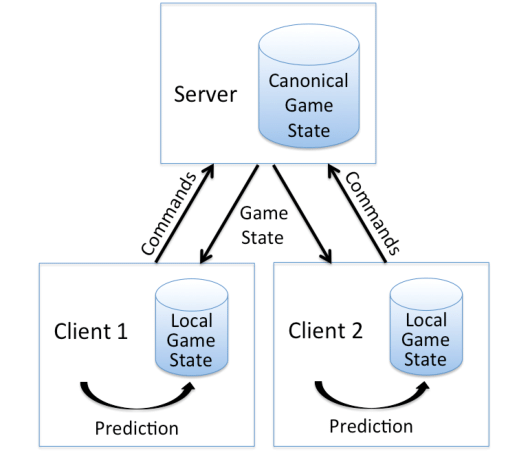
\includegraphics[width=10cm]{ClientServer}
	\caption{Kliens-Szerver architektúra}
	\label{fig-clientserver}
\end{figure}

A kliens és a szerver megbízható hálózati protokoll (pl. TCP vagy UDP) segítségével kommunikál, és olyan csomagokat küld, amelyek a játékosok interakcióiról, játékeseményekről és állapotfrissítésekről tartalmaznak információkat. 
 
Végső sorban szerver ellenőriz minden interakciót és csak ő tud dönteni a változásokról. Ez azért jó, mert így a csalásokkal szemben is védekezik a játék. 

Mivel mindig várni kell a szerver által küldött információra egy interakció esetén, így késleltetés léphet fel, főleg lassabb internet kapcsolat esetén. Erre egy módszer amit alkalmazni szoktak a klienseknél az úgynevezett predikció, ahol a helyi interakció alapján a kliens megpróbálja kitalálni mi fog ténylegesen történni \cite{MediumClientServer}.

\subsection{Peer-to-Peer (P2P)}

A P2P architektúra lényege, hogy a játékosok közvetlen kapcsolatot létesítenek egymással, így nincs szükség központi szerverekre, ellentétben a Kliens-Szerver architektúránál. Ebben a felépítésben, minden játékosnak helyi szinten kezeli a rendszer a játéklogikát.

\begin{figure}[ht!]
	\centering
	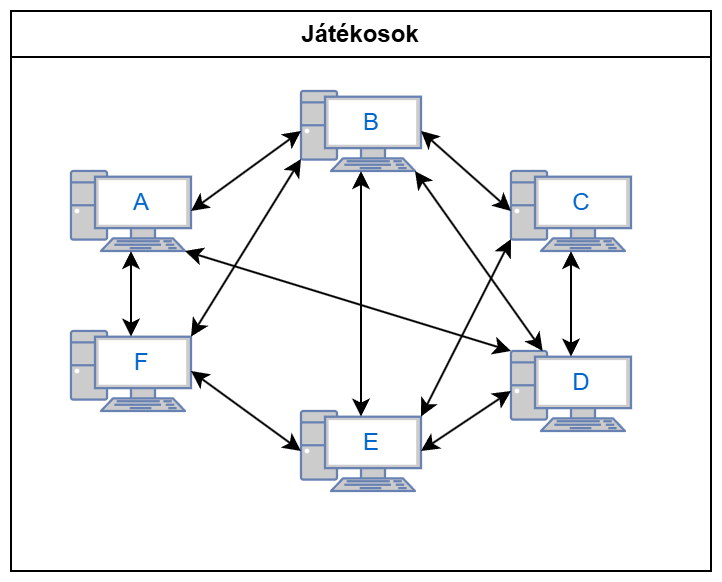
\includegraphics[width=10cm]{P2P}
	\caption{Peer-to-Peer architektúra}
	\label{fig-p2p}
\end{figure}

A P2P architektúra előnyei a Kliens-Szerver architektúrával szemben:
\begin{itemize}
	\item Mivel a játékosok közvetlen kapcsolatot alakítanak ki egymással, így általában gyorsabb a válaszidő.
	\item Sokkal költség hatékonyabb megoldás, mivel nem kell egy központi szerver üzemeltetésére költeni.
\end{itemize}

Mivel ebben a felépítésben nincs egy központi szerver, ami ellenőrző szerepet is tölt be, így a csalások kiszűrése több gondot okozhat. Mint minden felépítésnek, ennek is vannak előnyei és hátrányai is. Ezt az architektúrát kisebb játékos létszám igényű játékoknál célszerű használni. A szakdolgozatom során egy a Unity Technologies által létrehozott P2P architektúrán alapuló technológiát alkalmazok, amiről \aref{sec-relay}. fejezetben bővebben írok \cite{MediumP2P}.

\chapter{Unity}
\label{ch-unity}

A Unity egy játékmotor, amit aktívan a Unity Technologies fejleszt. A játékmotor segítségével számos platformra fejleszthetünk 2D és 3D játékokat is. Ezek a platformok közé tartoznak a virtuális valóságot szolgáltató platformok is. A megszokott asztali számítógépek mellett, mobil és web támogatást is nyújt a játékmotor \cite{UnityPlatforms}.

\section{Unity6}

Mai legfrissebb verziója a játékmotornak a Unity6, amit 2024 végén adtak ki. A frissítés számos nagy fejlesztéssel állt elő, amik közül nekem az egyik legfontosabb a tesztelés szempontjából, a \emph{Multiplayer play mode} volt. Fontosabb fejlesztések: 

\begin{itemize}
	\item Renderelés teljesítményének növelése
	\item Magával ragadóbb vizuális megjelenítés
	\item Többjátékos játékok fejlesztésének egyszerűsítése
	\begin{itemize}
		\item Multiplayer Center: kiválaszthatjuk, hogy milyen igényeink vannak a játékkal kapcsolatban, majd a Unity felsorolja nekünk a megfelelő technológiákat és csomagokat, így nem nekünk kell keresgélnünk és kutatnunk a csomagok után.
		\item Multiplayer Play Mode: talán ez volt számomra a legfontosabb, hiszen exponenciális mértékben felgyorsította a tesztelés folyamatát. A Multiplay Play Mode lehetővé teszi, hogy egyszerre több példányban is futhasson a játék a gépemen buildelés nélkül.
	\end{itemize}
	\item Web alapú fejlesztés teljesítményének növelése
	\item Gyorsított UI fejlesztés
\end{itemize}

Ezek mellett még számos fejlesztést és javítást hozott a frissítés \cite{Unity6Features}.

\section{Scene}

A játékok Unity-ben különböző jelenetekre (scene) vannak felbontva. A különböző jelenetekkel játékbeli tereket választhatunk el, például 1-1 szintet a játékon belül. A jeleneteken belül a játék fő építő eleme a \emph{GameObject}, amit egy fa hierarchiában tudunk a jelenetekbe pakolni \cite{UnityScene}.

\section{GameObject}
\label{sec-gameobject}

Unity-ben minden objektum egy GameObject. Ez azt jelenti, hogy mindennek, ami a játékban szerepelhet, GameObject-nek kell lennie. Önmagában egy GameObject nem csinál semmit, ezért tulajdonságokkal kell felruháznunk. A GameObject egy konténer, amihez darabokat adhatunk, amitől hang, effekt, karakter vagy akármi lehet. Ezeket a darabokat komponenseknek nevezzük \cite{UnityGameObjects}.

\subsubsection{Komponensek}

A komponensek lehetnek beépítettek, amivel a Unity szolgál, vagy akár írhatunk saját komponenseket C\# script-ek segítségével. Komponensek segítségével tudjuk életre kelteni a GameObject-eket. A saját script-ek írása lehetővé teszi a GameObject-en szereplő többi komponens módosítását és kezelését is. Komponenseket tudunk törölni és hozzáadni egy objektumhoz, ezeket a műveletek \aref{sec-editor}. fejezetben említett inspector ablakon keresztül tudjuk kezelni. Ebben a szekcióban bemutatom részletesebben a leggyakrabban használt komponenseket \cite{UnityComponents}.

\paragraph{Transform}

Az egyik legfontosabb komponens, amivel minden objektumnak rendelkeznie kell. Ezt a komponenst nem is lehet törölni az objektumokról. Információt szolgáltat az objektum: pozíciójáról, méretéről, forgásáról és a hierarchiában lévő tulajdonságairól is \cite{UnityTransform}.
	
\paragraph{RigidBody}

Azok az objektumok amelyeken van ilyen komponens, azok használják a beépített fizikai motort a gravitáció és többi fizikai hatás szimulálásához. A Transform komponens használata helyett, a fizikai motor segítségével módosítható az objektum pozíciója. Különféle fizikai hatásokat szimulálhatunk a komponens segítségével. Számos tulajdonságot is beállíthatunk az objektumnak, mint például a tömegét, a pontosabb szimulációk érdekében \cite{UnityRigidbody}.

\paragraph{Camera}

A játékos a kamerán keresztül fogja látni a világot. Egy projekt létrehozásakor alapból létrejön egy objektum, amire a Camera komponens már hozzá van adva. A komponensen különféle beállításokat találhatunk a felbontással, effektekkel és hasonlókkal kapcsolatban \cite{UnityCamera}.

\paragraph{Collider}

Ez a komponens lehetőséget ad két objektum találkozásának vizsgálatára. Ha mozgatni is szeretnénk az objektumokat, akkor RigidBody használatával tudjuk csak megtenni. Több különböző formában tudjuk az objektum köré tenni: \cite{UnityCollider}

\begin{itemize}
	\item Box (3D)
	\item Square (2D)
	\item Sphere (3D)
	\item Circle (2D)
	\item Mesh (3D)
	\item Polygon (2D)
\end{itemize}

\paragraph{Sprite Renderer}

Ez a komponens lehetővé teszi a képek megjelenítését 2D illetve 3D projektekben is. Egy sprite-ot kell megadnunk neki, amit különböző képformátumokból a Unity-be importálva tudunk létrehozni \cite{UnitySpriteRenderer}.

\paragraph{Light}

Ennek a komponensnek a segítségével tudjuk kezelni a fényeket a játékban. 2D és 3D esetén is több különböző light komponenst szolgáltat a Unity. A fényeknek lehetőségünk van állítani a fényét, színét, távolságát és még sok hasonló tulajdonságot \cite{UnityLight}.

\paragraph{Audio Source}

Ennek a komponensnek egy Audio Clip-et szolgáltatva tudjuk lejátszani az adott hangunkat. Van lehetőségünk a hangerőt és hasonló tulajdonságokat módosítanunk. Használatához szükségünk van egy Audio Listener komponensre is, aminek segítségével akár térben is különbséget tehetünk a hangok között \cite{UnityAudioSource}.

\paragraph{Script}

Az egyik legfontosabb komponens, amivel személyre tudjuk szabni a játékmenetet. Mindegyik script megírása C\#-ban történik. Az olyan script-ek amiket egy objektumhoz akarunk kötni a MonoBehaviour beépített osztályból kell örököltetnünk. Ez az osztály sok különböző metódust és függvényt ad, de ezek közül a 2 legfontosabb a start és az update metódusok.

\begin{itemize}
	\item Start: a start metódus egyszer fut le, amikor az objektum betölt a játékba.
	\item Update: az update metódus minden frame-ben lefut, amikor az objektum aktív.
\end{itemize}

A megírt kódban különböző objektumokra és komponensekre is tudunk hivatkozni, amit \aref{sec-editor}. fejezetben említett inspector ablakban kell be referálnunk. Lehetőségünk van másik script-re is hivatkozni. A játékfejlesztésben sok tervezési minta megtalálható az optimális kód írására, de a leggyakrabban használtnak mondható az egyke (singleton) tervezési minta \cite{UnityScripting}.

\section{Prefab}
\label{sec-prefab}

A Unity Prefab rendszere lehetővé teszi egy GameObject el tárolását, minden komponensével, tulajdonságértékével és gyermek GameObjectjével együtt, egy újrafelhasználható objektumként. Ha van egy olyan objektumunk, amit sokszor újra fel szeretnénk használni a jelenteinkben, akkor érdemes Prefab-et használni ezeknek az objektumoknak az eltárolására. Egyes Prefab-ek esetén felülírhatjuk az alap beállításokat, így kis szinten különböző de logikailag összefüggő objektumokat használhatunk. Néhány gyakori példa a Prefab használatra: \cite{UnityPrefab}

\begin{itemize}
	\item Nem játékos karakterek (NPC-k) - akár egy ellenfél típussal többször is találkozhatunk a játékunk során.
	\item Lövedékek - például egy ágyú esetén, az ágyú golyó maga lehet egy Prefab, ami minden tüzelés során létrejön.
	\item Ismétlődő UI elemek - például Játékos kártyák egy lobby panelen.
\end{itemize}

\section{Editor}

\label{sec-editor}
Minden ami nem kód írás egy játék fejlesztése során, az az editor-ban fog történni. A Unity editor több különböző ablakból tevődik össze, amik segítik a fejlesztési folyamatot. Ebben a szekcióban bemutatom részletesebben a legfontosabb ablakokat.

\begin{figure}[ht!]
	\centering
	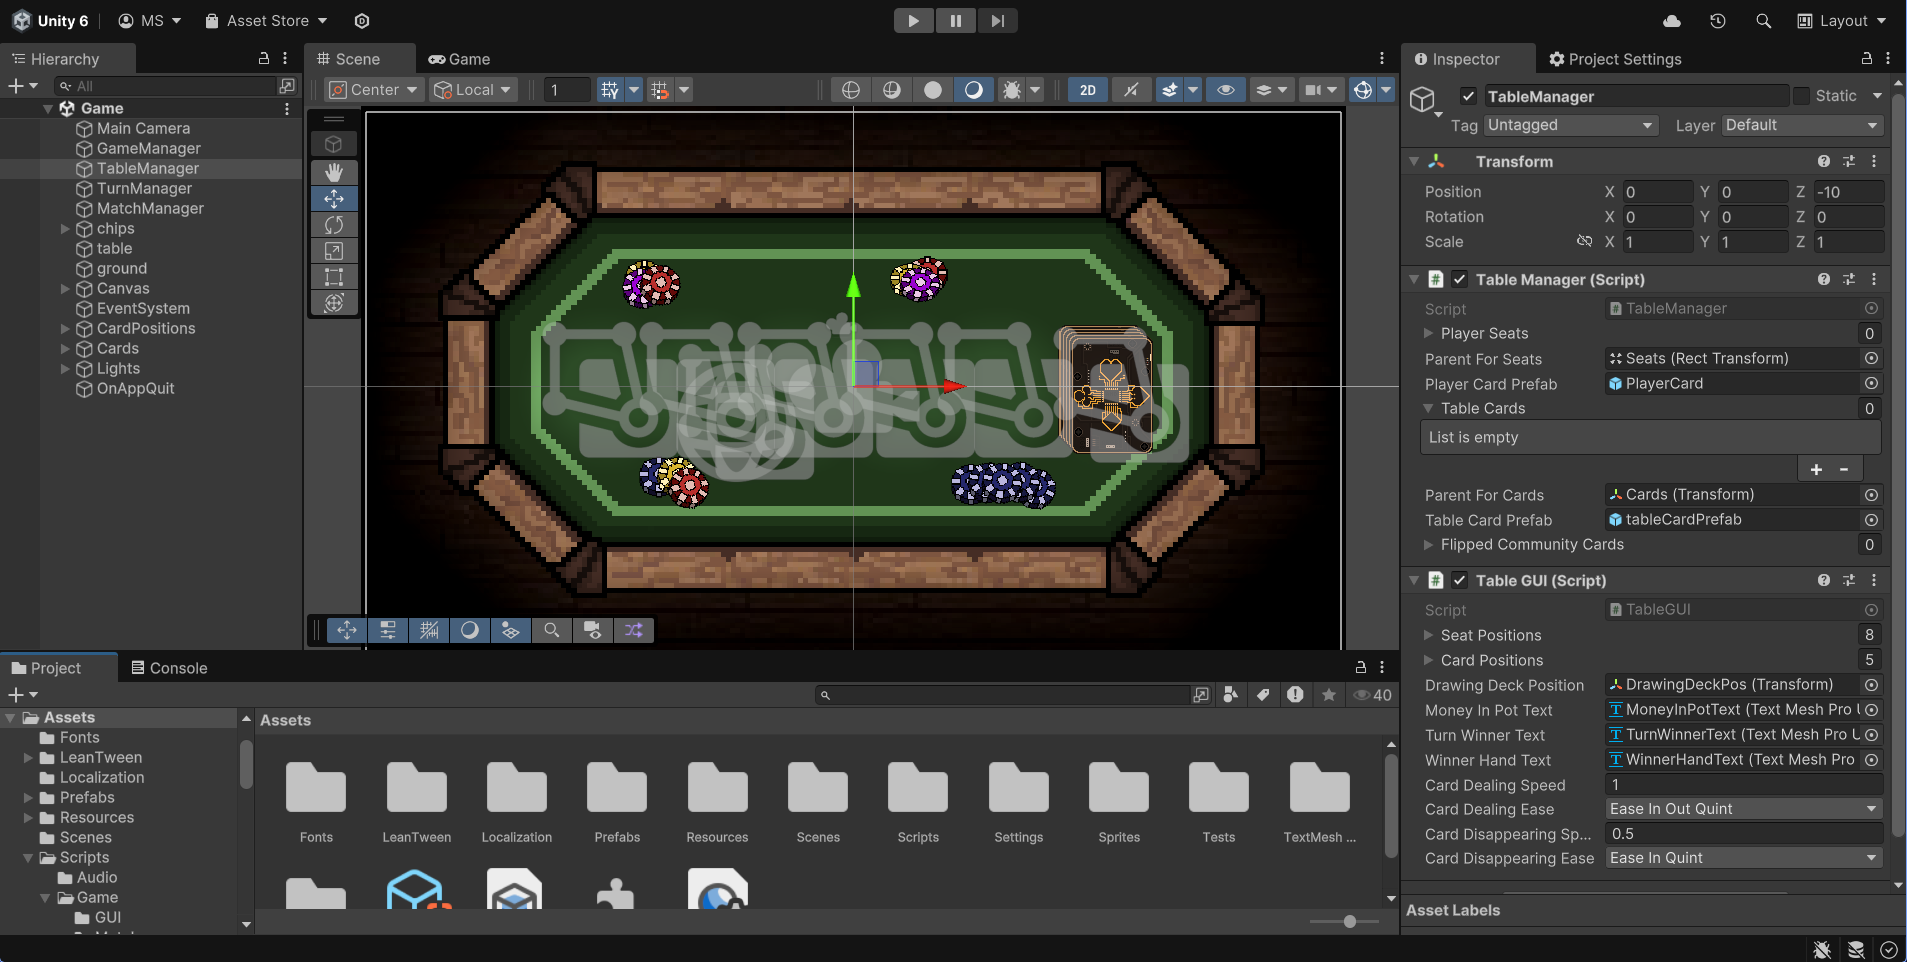
\includegraphics[width=15cm]{UnityEditor}
	\caption{Unity editor}
	\label{fig-unityeditor}
\end{figure}

\paragraph{Project Window}

Ebben az ablakban tudjuk kezelni a fájlrendszerét a projektünknek. Itt hozhatunk létre rendszerezés céljából különböző mappákat, és helyezhetjük el a felhasználni kívánt fájlokat is \cite{UnityProjectWindow}.

\paragraph{Scene View}

Ez az egyik legfontosabb ablak. Itt tudjuk kezelni a jeleneten belüli játék elemeinket. Több különböző módon tudjuk manipulálni az objektumokat, beleértve a pozíciójuk módosítását, és az átméretezésüket is \cite{UnitySceneView}.

\paragraph{Hierarchy Window}

Ez az ablak tartalmazza a jelenlegi jeleneten belüli összes játék objektumot. Itt tudunk létrehozni új objektumokat, és a faszerű hierarchia nézetben rendezni őket \cite{UnityHierarchyWindow}.

\paragraph{Inspector Window}

Ha kiválasztunk egy objektumot a hierarchiában, vagy a jelenet nézetben, akkor azt az objektumot ezen az ablakon keresztül tudjuk kezelni. Itt tudunk új komponenseket adni hozzá és a meglévőeket pedig módosítani. Itt tudjuk például a saját kódjainkat is az objektumokra helyezni \cite{UnityInspectorWindow}.

\paragraph{Game View}

Ezen az ablakon látható a játékban használt kamerák által rögzített renderelt kép, amely a végső játékot mutatja be \cite{UnityGameView}.

\section{Relay}

\label{sec-relay}
A Relay szolgáltatás lehetőséget ad arra, hogy többjátékos játékokat fejlesszünk drága dedikált szerverek nélkül. A kapcsolódás folyamat hozzáférési kódokon keresztül történik a játékosok között. A Unity Technologies elmondása szerint ezt a szolgáltatást kis méretű casual játékokhoz és kör alapú kártya játékokhoz a legérdemesebb használni. Az alábbiak a fő előnyei ennek a szolgáltatásnak \cite{UnityRelayService} \cite{UnityRelayDocs}.

\begin{itemize}
	\item Költséghatékony megoldás a játékosok összekapcsolásra: A Peer-to-Peer alapú megoldás lehetővé teszi, hogy a játékosok a saját eszközeiken hosztolják a játékot és így nincs szükség drága szerverekre.
	\item Automatikus és egyszerű skálázás: a Relay kezeli nekünk a skálázási igényeket, akár 100 játékost is képes összekapcsolni egy játékmenetbe.
	\item Biztonságos kapcsolat: a Relay kezeli helyettünk a biztonságos kapcsolatot és biztosítja az információk titkosított cseréjét a játékosok között.
\end{itemize}

Két fő komponensből épül fel a Relay.

\begin{itemize}
	\item Relay Server: az alacsony szintű Unity Transport réteghez kapcsolódik, hogy bájtokat küldjön a játékosok között. Ennek segítségével a játékomban fix bájton tárolt szöveges adatokat küldök a játékosok között, aminek a pontosabb menetéről a \aref{sec-tobbjatekoskapcsolat}. fejezetben bővebben írok.
	\item Relay Allocation Service: backenden működik, hogy a játékosok a hozzáférési kódok megosztásával játékmeneteket hozhassanak létre és csatlakozhassanak hozzájuk \cite{UnityAllocationsService}.
\end{itemize}

\subsection{Relay Server}

A játékosok nem közvetlen egymáshoz csatlakozva, hanem Relay szervereken keresztül kommunikálnak egymással. A Relay szerverek továbbítják az üzeneteket a kliensek között kis késleltetésű datagram cserével, ez biztosítja azt, hogy két játékos sose kapcsolódik közvetlen egymáshoz. Ezek a szerverek nyilvános végpontként viselkednek, ami elérhető az összes játékos számára. Ez a megközelítés megoldást ad több különböző felmerülő problémára is mint például a játékosok közötti tűzfalakra. Minden játékos ugyanarra az ip címre tud csatlakozni, amit biztosra vehetnek, hogy a játékmenet során nem fog változni, így a játékosoknak nem kell tudniuk egymás ip címéről, ez is erősíti a biztonságot a rendszerben \cite{UnityRelayServers}.

\begin{figure}[ht!]
	\centering
	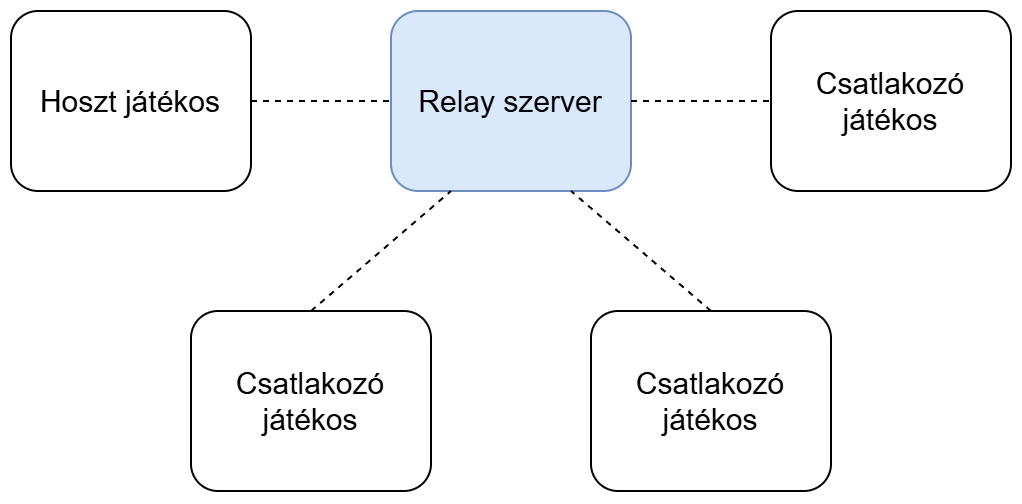
\includegraphics[width=10cm]{RelayServer}
	\caption{Relay szerverek felépítése}
	\label{fig-unityrelayservers}
\end{figure}

\chapter{Rendszerterv}
\label{ch-rendszerterv}

\section{Rendszer célja}

A szakdolgozatom célja egy Texas Hold'Em szabályain alapuló póker játék fejlesztése, ahol egy asztali számítógép és több mobiltelefon között jön létre a kapcsolat a többjátékos játékmenet megvalósításához. A játék célja, hogy egy hasonló élményt adjon a játékosok számára, mintha rendes pókert játszanánk élőben. Ezt a célt úgy próbáltam elérni, hogy a mobiltelefonok képzik a játékosok ,,kezeit'' és a számítógép pedig az asztalt, az az a közös teret.

\section{Architekturális terv}
\label{sec-architecture}

A szakdolgozat 3 különböző projektből épül fel: PC játék (Unity), Mobil játék (Unity), Közös DLL (C\# Class Library). Mivel mind a három projekt a C\# programozási nyelvet használja, így egyszerűen lehet kezelni a közös metódusokat, könyvtárakat, funkciókat.

\paragraph{PC játék}

A PC játék szolgál az asztalként, itt lehet létrehozni és kezelni a játszmákat. A játékmenet fontosabb részei itt nyomon követhetők a játékosok számára. 

\paragraph{Mobil játék}

A Mobil játék szerepe a PC-s játékkal való kommunikáció megteremtése a játékosok számára. A játékosok itt tudnak különféle üzenetek küldésével játszani a játékkal, miközben a játékmenet többi részét a PC-n követhetik.

\paragraph{Közös DLL}

A közös DLL szerepe azoknak a függvényeknek és metódusoknak összegyűjtése, amit mind a PC illetve a Mobil játék során is használok a kódban. Ennek egyik legfontosabb része a kézkiértékeléshez szükséges algoritmus, amiről bővebben \aref{subsec-kezkiertekeloalgoritmus}. fejezetben írok. A DLL-nek egy másik fontos része a két játék közötti üzenetek egységbe fogása. Az üzenetek küldéséről \aref{sec-tobbjatekoskapcsolat}. fejezetben bővebben írok, de a lényeg, hogy az üzenet küldés során használt osztályokat is a DLL tartalmazza, hiszen így mindkét oldal egységesen tudja kezelni őket.

\section{Követelmények}

Ebben a szekcióban a szakdolgozat sikeres kivitelezéséhez szükséges követelményekről írok részletesen.

\subsection{PC játék}

A PC játék rendelkezik egy főmenüvel, amelyen keresztül kezelhetőek a beállítások, illetve innen indítható új játék. A főmenüből létrehozott új játék során először egy Lobby felület jelenik meg.

\subsubsection{Beállítások}


\begin{table}[ht!]
	\centering
	\footnotesize
	\begin{tabular}{|p{3cm}|p{7cm}|p{4cm}|}
		\hline
		\textbf{Funkció} & \textbf{Leírás} & \textbf{Opciók/Példák} \\ 
		\hline
		Felbontás & A játék képernyőfelbontásának kiválasztása & 1920x1080, 1280x720, stb. \\ 
		\hline
		Grafikai minőség & Grafikai részletesség és effektusok beállítása & Alacsony, Közepes, Magas \\ 
		\hline
		SFX Hangerő & Játék hangerejének szabályozása & 0–100\% \\ 
		\hline
		Zene Hangerő & Játék hangerejének szabályozása & 0–100\% \\ 
		\hline
	\end{tabular}
	\caption{Beállítási felület követelményei}
\end{table}

\subsubsection{Lobby}

A Lobby felületen megjelenik a hozzáférési kódot, amivel a játékosok a mobiljukról tudnak csatlakozni a játszmához.

\begin{table}[ht!]
	\centering
	\footnotesize
	\begin{tabular}{|p{3cm}|p{7cm}|p{4cm}|}
		\hline
		\textbf{Funkció} & \textbf{Leírás} & \textbf{Opciók/Példák} \\ 
		\hline
		Játékosok megjelenítése & Csatlakozott játékosok listázása (név, státusz) & ,,Játékos1 - készen áll'' \\ 
		\hline
		Játékos kirúgása & A játékos eltávolítása a lobby-ból (csak a host számára) & ,,Kirúgás'' gomb \\ 
		\hline
		\raggedright Hozzáférési kód megjelenítése & Egyedi azonosítókód mutatása, amelyet a játékosok használnak a csatlakozáshoz & ,,ABC123'' \\ 
		\hline
		Státuszok jelzése & Jelzés, hogy ki áll készen a játék indítására & Készen áll / Nincs kész \\ 
		\hline
		Chat-funkció & Kommunikáció a lobby játékosai között & Chat-ablak,\newline,,Játékos1: üzenet'' \\ 
		\hline
		Kezdő pénz beállítása & A host választhat különböző kezdőértékek közül & 100\$, 250\$, 500\$ \\ 
		\hline
		Játékindítás & A host elindíthatja a játékot, ha mindenki készen áll & ,,Indítás'' gomb \\ 
		\hline
	\end{tabular}
	\caption{Lobby felület követelményei}
\end{table}

\subsubsection{Játék}

Miután a Lobby-ból elindítottuk a játékot, betölt egy új jelenetet, ahol az asztal látszódik, és a becsatlakozott játékosok körben helyezkednek el az asztal körül. A játék során a következő funkciók jelennek meg és állnak rendelkezésre:

\begin{table}[ht!]
	\centering
	\footnotesize
	\begin{tabular}{|p{3cm}|p{7cm}|p{4cm}|}
		\hline
		\textbf{Funkció} & \textbf{Leírás} & \textbf{Opciók/Példák} \\ 
		\hline
		\raggedright Játékos megjelenítése & Játékos megjelenítése UI elemek segítségével & Kártya, ahol látszik a játékos neve és pénze \\
		\hline
		Aktív játékos kijelzése & Világosan látható, hogy ki következik a körben & Játékos1 kártyájának kiemelése \\ 
		\hline
		Legutóbbi esemény & Látszik az adott játékos kártyáján, hogy mit csinált legutóbb & ,,Emelt 50\$-ral'' \\
		\hline
		Kártyák osztása az asztalra & Kártyák automatikus kiosztása a megfelelő pillanatban & Kártyák csúsztatása egyesével az asztalra animációval \\ 
		\hline
		\raggedright Kártyák felfordítása & Kártyák automatikus felfordítása a megfelelő pillanatban & Kártyák felfordítása egyesével az asztalon \\ 
		\hline
		Kártyák osztása játékosoknak & Kártyák automatikus kiosztása a megfelelő pillanatban & Kártyák csúsztatása egyesével a játékosoknak animációval \\ 
		\hline
		\raggedright Kör végének mutatása & Feljön egy ablak, ahol látszik ki nyerte meg a kört és milyen kézzel & ,,Játékos3 nyert:\newline Royal Flush'' \\
		\hline
		Játékos kezek mutatása & Minden játékosnak megjelenik milyen kártyák voltak a kezében & ,,Játékos2:\newline [Szív király, Gyémánt 10]'' \\
		\hline
		Nyertes mutatása & A játszma végén megjelenik a nyerő játékos neve egy felületen & ,,Játékos1 nyert'' \\
		\hline
		Visszalépés a főmenübe & A játszma végén vissza lehet lépni a főmenübe & ,,Visszalépés a főmenübe'' gomb \\
		\hline
	\end{tabular}
	\caption{Játék jelenet követelményei}
\end{table}

\subsection{Mobil játék}

A mobil játék kezdőképernyőjén lehetőségünk van egy játékos név és egy hozzáférési kód megadásával csatlakozni egy adott játszmához.

\begin{table}[ht!]
	\centering
	\footnotesize
	\begin{tabular}{|p{3cm}|p{7cm}|p{4cm}|}
		\hline
		\textbf{Funkció} & \textbf{Leírás} & \textbf{Opciók/Példák} \\ 
		\hline
		\raggedright Játékos név megadása & Játékos név megadására ad lehetőséget egy szerkeszthető szövegdoboz segítségével & ,,Játékos1'' \\ 
		\hline
		\raggedright Hozzáférési kód megadása & Hozzáférési kód megadására ad lehetőséget egy szerkeszthető szövegdoboz segítségével & ,,ABC123'' \\ 
		\hline
		\raggedright Csatlakozás játékhoz sikeres & A megadott információkkal megpróbál egy játékhoz csatlakozni & ,,Csatlakozás'' gomb \\ 
		\hline
		\raggedright Csatlakozás játékhoz sikertelen & Kijelzi az okát a sikertelen csatlakozásnak & ,,A megadott hozzáférési kóddal játszma nem található'' \\ 
		\hline
	\end{tabular}
	\caption{Kezdőképernyő követelményei}
\end{table}

\subsubsection{Lobby}

Sikeres csatlakozás után a Lobby felület jelenik meg. A Lobby felületen tudunk üzenetet küldeni a többi játékos számára, kilépni a játszmából és a készenléti állapotot módosítani.

\begin{table}[ht!]
	\centering
	\footnotesize
	\begin{tabular}{|p{3cm}|p{7cm}|p{4cm}|}
		\hline
		\textbf{Funkció} & \textbf{Leírás} & \textbf{Opciók/Példák} \\ 
		\hline
		Chat üzenet küldése & Chat üzenet küldés, ami a PC játékon megjelenik, hogy minden játékos lássa & ,,Játékos1: üzenet'' \\ 
		\hline
		\raggedright Készenlét módosítása & Készenlét be és ki kapcsolása & ,,Készen állok'', ,,Nem állok készen'' gombok \\ 
		\hline
		Kilépés a játszmából & Kilépés a csatlakozott játszmából & ,,Kilépés'' gomb \\ 
		\hline
	\end{tabular}
	\caption{Lobby felület követelményei}
\end{table}

\subsubsection{Játék}

Ha az összes játékos készen állt, és a PC-n elindította a hoszt a játszmát, akkor egy új jelenet tölt be, ahol a játszma során tudjuk kezelni az interakcióinkat. Ez a jelenet 2 felületből épül fel: akciók felület, kártyák felület. Az egyik felületen tudja kezelni a játékos a lépéseit a másik felületen pedig megtudja nézni a neki kiosztott kártyákat.

\begin{table}[ht!]
	\centering
	\footnotesize
	\begin{tabular}{|p{3cm}|p{7cm}|p{4cm}|}
		\hline
		\textbf{Funkció} & \textbf{Leírás} & \textbf{Opciók/Példák} \\ 
		\hline
		Pénz megjelenítése & A játékos jelenlegi pénze megjelenik a felületen & ,,Pénz: 50\$'' \\ 
		\hline
		2 felület közötti váltás & Váltás az akciók és a kártyák felület között & ,,Kártyák megjelenítése'',\newline ,,Akciók megjelnítése''\newline gombok \\ 
		\hline
		\raggedright Akciók felület (a játékos következik) & Lehetséges akciók megjelenítése & ,,Bedobás'', ,,All In'' gombok, Tét megadására szolgáló csúszka, stb\dots \\ 
		\hline
		\raggedright Akciók felület (nem a játékos következik) & Figyelmeztető üzenet megjelenítése & ,,Nem a te vagy jelenleg a körben'' \\ 
		\hline
		\raggedright Kártyák felület (van kártya a játékos kezében) & Kártyák megjelenítése és a legjobb használható kéz feltüntetése & A 2 kártyáról 1-1 kép,\newline ,,Legjobb kéz: Kettes pár'' felirat \\ 
		\hline
		\raggedright Kártyák felület (nincs kártya a játékos kezében) & Figyelmeztető üzenet megjelenítése & ,,Nincs kártya a kezedben'' \\ 
		\hline
		Kilépés a játszmából & Kilépés a csatlakozott játszmából & ,,Kilépés'' gomb \\ 
		\hline
	\end{tabular}
	\caption{Játék jelenet követelményei}
\end{table}

\section{Használt fejlesztői eszközök}

A fejlesztés folyamatát számos eszköz segítette és gyorsította fel. Ebben a szekcióban ezeket az eszközöket sorolom fel, és ismertetem röviden. A fejlesztésnek nem csak a kódolás a része, így látható lesz, hogy több különböző eszköz, amiknek nincs közük a kódoláshoz is segítették a fejlesztést.

\paragraph{Unity}

A Unity az első és talán legfontosabb eszköz, ami az alapját adta a 2 játéknak. Erről a játékmotorról már korábban \aref{ch-unity}. fejezetben írtam.

\paragraph{Rider}

A Rider egy a JetBrains által fejlesztett integrált fejlesztői környezet, aminek segítségével különböző .NET projekteket és játék projekteket tudunk fejleszteni. Egy cross-platform IDE, az az több különböző platformon is elérhető számunkra. A környezet beépített Unity támogatással rendelkezik, és különböző funkciókat szolgáltat a C\# szkriptek írásának megkönnyítésére \cite{Rider}.

\paragraph{Git, GitHub}

A Git egy nyílt forráskódú, verziókezelő rendszer, amely lehetővé teszi a projektek forráskódjának és fájljainak változásainak nyomon követését. A Git segítségével hatékonyan lehet kezelni a változások történetét, különböző verziókat létrehozni, valamint a kollaboráció során fellépő konfliktusokat egyszerűbben megoldani. A GitHub egy online platform, amely a Git verziókezelő rendszerre épül, és számos hasznos szolgáltatást nyújt, mint például távoli tárolók (repository-k) létrehozása. A GitHub lehetővé teszi a kód egyszerű megosztását, és elérését különböző helyekről \cite{Git} \cite{GitHub}.

\paragraph{Trello}

A Trello egy vizuális, online projektmenedzsment eszköz, amely segítségével egyszerűen és átláthatóan kezelhetőek különböző feladatok és munkafolyamatok. A Trello kártyákon alapuló rendszerében egyes feladatokat vagy tennivalókat kártyákként kezelhetünk, amelyeket különböző listákba rendezhetünk, például ,,Teendő'', ,,Folyamatban'', vagy ,,Kész''. Ezáltal könnyen áttekinthető, hogy hol tartunk, és hogy mi van még hátra a projektünkből \cite{Trello}.

\chapter{Saját szoftver megvalósítása}

\section{Texas Hold'Em}

A póker a világ egyik legismertebb kártyajátéka, amelyben a játékosok célja, hogy a saját lapjaikból a lehető legjobb kombinációt kialakítva megszerezzék az asztalon lévő kasszát. A póker számos különböző szabályrendszerrel rendelkező változatban létezik.

A \emph{Texas~Hold’Em} a közösségi pókerjátékok legnépszerűbb formája, amelyet jellemzően 2 és 10 játékos között játszanak. Ez egy viszonylag zárt struktúrájú játék, ahol a licitálás menete állandó szabályok szerint zajlik.

\subsection{Szabályok ismertetése}
\label{subsec-pokerszabalyok}

Ebben a szekcióban a póker legelterjedtebb, hivatalos versenyeken is alkalmazott szabályrendszere kerül bemutatásra. Ami közös az összes variációban, hogy a játékot 52~lapos francia kártyával játsszák dzsókerek nélkül.

\subsubsection{Játék menete}

A játék során három fontos szerep forog körbe a játékosok között, amit ,,gombokkal'' jelölünk. Ezek a szerepek az osztó, kis vak és nagy vak. Az osztótól balra ülő játékos lesz a kis vak, a kis vaktól balra ülő pedig a nagy vak. Az osztót pedig több különböző módon választhatjuk meg a játék elején.  

Az osztó keveri és osztja ki a lapokat a szabályok szerint. A vakok pedig még osztás előtt kötelesek betenni a vak téteket, ahol a kis vak tét általában a nagy vak tét fele. Egy játszma az alábbiak szerint játszódhat le: \cite{TexasholdemSzabalyok}

\begin{enumerate}
	\item \emph{Osztás}
	\begin{itemize}
		\item Az osztó először megkeveri a paklit. A kiosztás előtt a kis vak és a nagy vak beteszik a kötelező téteket. Ezt követően az osztó balról kezdve, két körben, egyesével oszt minden játékosnak egy-egy zárt lapot.
	\end{itemize}
	\item \emph{Pre-Flop (első licitkör)}
	\begin{itemize}
		\item A licitálás a nagy vaktól balra ülő első játékossal kezdődik, aki az alábbi lehetőségek közül választhat:
		\begin{itemize}
			\item Tartás -- megadja az aktuális tétet.
			\item Emelés -- növeli a tétet a limitszabályok szerint.
			\item Dobás -- eldobja a lapjait, ezzel kiszáll a játékból.
		\end{itemize}
		\item A licitálás az óramutató járásával megegyező irányban halad tovább.
	\end{itemize}
	\item \emph{Flop (második licitkör)}
	\begin{itemize}
		\item Az osztó egy lapot félretesz égető lapként, majd három közös lapot felfordítva az asztal közepére helyez.
		\item A licitálást az osztógombtól balra ülő első aktív játékos kezdi, és az alábbi lehetőségek közül választhat:
		\begin{itemize}
			\item Passzolás -- nem emel, de marad a játékban.
			\item Nyitás -- tétet tesz be a limitszabályok szerint.
			\item Dobás -- eldobja a lapjait és kiszáll a körből.
		\end{itemize}
		\item Ha valaki nyit, a többiek dönthetnek:
		\begin{itemize}
			\item Tartás -- megadják a tétet.
			\item Emelés -- növelik a tétet.
			\item Dobás -- kiszállnak a körből.
		\end{itemize}
	\end{itemize}
	\item \emph{Turn (harmadik licitkör)}
	\begin{itemize}
		\item Az osztó ismét éget egy lapot, majd egy negyedik közös lapot felfordítva az asztalra helyez.
		\item A harmadik licitkör a második licitkörhöz hasonlóan zajlik.
	\end{itemize}
	\item \emph{River (negyedik licitkör)}
	\begin{itemize}
		\item Az osztó még egy égető lapot félretesz, majd kiosztja az utolsó, ötödik közös lapot.
		\item Minden játékos hét lapból próbálja a lehető legjobb ötlapos kombinációt kialakítani.
		\item Az utolsó licitkör a második és a harmadik licitkörhöz hasonlóan zajlik.
	\end{itemize}
	\item \emph{Showdown (lapok felfedése)}
	\begin{itemize}
		\item Ha az utolsó licitkör után egynél több játékos marad, akkor a játékosok megmutatják a lapjaikat választásuk szerint.
		\item A kasszát a legerősebb pókerkezet birtokló játékos nyeri el.
	\end{itemize}
\end{enumerate}

\subsubsection{Pókerkezek}

Az alábbi felsorolás a lehetséges pókerkezeket mutatja be, amelyeket erősségük szerint rendeztem el, a legerősebbtől a leggyengébbig. A lista tetején található kéz a pókerben elérhető legmagasabb értékű kombináció, és innen lefelé haladva egyre gyengébb kezek következnek. Az alábbi sorrend megtekinthető \aref{fig-pokerhands}.~ábrán is \cite[9.~oldal]{Szurdi}.

\begin{enumerate}
	\item \emph{Royal flös (royal flush)}: A legerősebb lapkombináció. Egyszínű 10-es, bubi, dáma, király, ász lapokból áll. Ha két ilyen találkozik, akkor döntetlen\footnote{Osztozás történik a nyeremény között.} van.
	
	\item \emph{Színsor (straight flush)}: Öt egyszínű sorba rendezhető lapból áll. Ha két ilyen találkozik, a legmagasabb lap dönt. Ha egyforma, akkor döntetlen van. 

	\item \emph{Póker (four of a kind)}: Négy ugyanolyan számozású vagy jelű lapból és egy akármilyen másik lapból áll. Ha két ilyen találkozik, a magasabb póker nyer.

	\item \emph{Full (full house)}: Három ugyanolyan számozású vagy jelű lapból és két másik ugyanolyan számozású vagy jelű lapból áll. Ha két ilyen találkozik, a magasabb drill nyer. Ha egyforma, a magasabb pár nyer.

	\item \emph{Szín (flush)}: Öt ugyanolyan színű lapból áll. Ha két ilyen találkozik, a legmagasabb lap dönt. Ha egyforma, a második legmagasabb dönt, és így tovább\dots

	\item \emph{Sor (straight)}: Öt sorba rendezhető lapból áll. Ha két ilyen találkozik, a legmagasabb lap dönt. Ha egyforma, a színerősség dönt.

	\item \emph{Drill (three of a kind)}: Három ugyanolyan számozású vagy jelű lapból és két akármilyen másik lapból áll. Ha két ilyen találkozik, a magasabb drill nyer. Ha egyforma, a magasabb semleges lap, majd az alacsonyabb dönt.

	\item \emph{Két pár (two pairs)}: Kétszer két ugyanolyan számozású vagy jelű lapból áll. Ha két ilyen találkozik, a magasabb pár, majd az alacsonyabb, majd a semleges lap erőssége dönt.

	\item \emph{Egy pár (one pair)}: Két ugyanolyan számozású vagy jelű lapból és három akármilyen másik lapból áll. Ha két ilyen találkozik, a magasabb pár nyer. Ha egyforma, a semleges lapok döntenek.

	\item \emph{Magas lap (high card)}: Bármilyen lap, abból is a legmagasabb értékkel rendelkező.
\end{enumerate}

\begin{figure}[ht!]
	\centering
	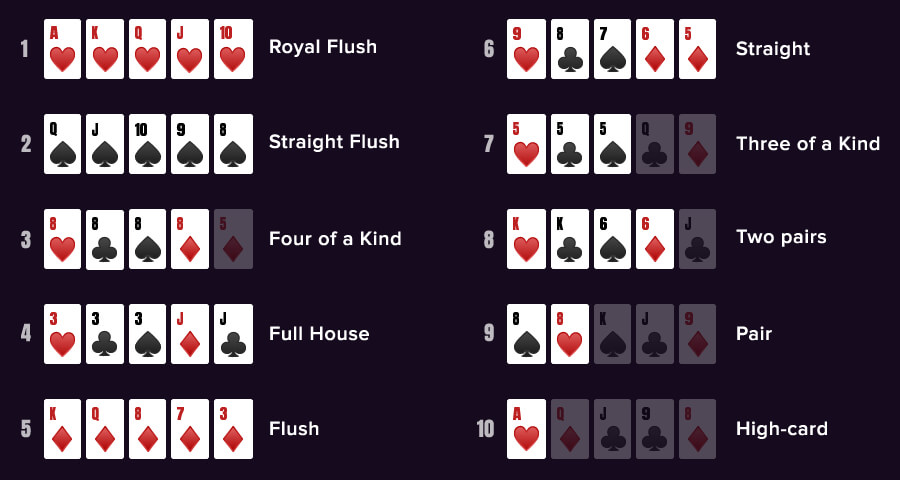
\includegraphics[width=14cm]{PokerHands}
	\caption{Lehetséges pókerkezek}
	\label{fig-pokerhands}
\end{figure}

\subsection{Használt kézkiértékelő algoritmus}
\label{subsec-kezkiertekeloalgoritmus}

A legelterjedtebb kézkiértékelő algoritmusok azon alapulnak, hogy a kezek értékeit egy előre kiszámított kéz értékeket tároló táblából keressük ki. Ez az egyik leggyorsabb módszer, viszont a módszer egy nagy hátránya a nagy méretű tábla tárolása, amely tárhely igényes. A játékomban egy bit matematikán alapuló algoritmust használtam, aminek alapjait \acite{HandEvaluation} blog adta. Ez a módszer lassabb, mint a táblás, viszont a tárhely igényes probléma itt megszűnik.

\subsubsection{Algoritmus}

Az alábbi lépéseket kell végrehajtanunk a kézkiértékeléshez:

\begin{enumerate}
	\item Minden kártyáról el kell tárolnunk a rangját és a színét. Az inputunk 5 darab ilyen kártyából fog állni.
	\item 2 különböző bitmező létrehozása a kártyák alapján
	\begin{itemize}
		\item Az első mező a kártyák rangjának előfordulásáról tartalmaz 15~biten információt. Az egyes biteken azt fogjuk jelölni, hogy az adott rangból van-e az 5 adott kártya között (1 ha van, 0 ha nincs). \Aref{tab-bitfieldvalues1} táblázatban és \aref{tab-bitfieldvalues2} táblázatban látható 1-1 példa az elő állított bitmezőről.
		
		\begin{table}[ht!]
			\centering
			\footnotesize
			\begin{tabular}{*{15}{c}}
				0 & 1 & 1 & 1 & 1 & 1 & 0 & 0 & 0 & 0 & 0 & 0 & 0 & 0 & 0\\
				A & K & Q & J & T & 9 & 8 & 7 & 6 & 5 & 4 & 3 & 2
			\end{tabular}
			\caption{[9, 10, J, Q, K] kártyákhoz tartozó első bitmező}
			\label{tab-bitfieldvalues1}
		\end{table}
		
		\begin{table}[ht!]
			\centering
			\footnotesize
			\begin{tabular}{*{15}{c}}
				0 & 1 & 0 & 0 & 0 & 1 & 0 & 0 & 0 & 0 & 0 & 0 & 0 & 0 & 0\\
				A & K & Q & J & T & 9 & 8 & 7 & 6 & 5 & 4 & 3 & 2
			\end{tabular}
			\caption{[9, 9, 9, K, K] kártyákhoz tartozó első bitmező}
			\label{tab-bitfieldvalues2}
		\end{table}
		
		\item A második mező a rangok előfordulásának számáról tárol információt 60~biten. Minden ranghoz rendelünk 4 bitet, ahol annyit jelölünk 1-el, amennyi darabunk van az adott rangból. \Aref{tab-bitfieldcounts1} táblázatban és \aref{tab-bitfieldcounts2} táblázatban látható 1-1 példa az elő állított bitmezőről.
		
		\begin{table}[ht!]
			\centering
			\footnotesize
			\begin{tabular}{*{8}{r}}
				0000 & 0001 & 0001 & 0001 & 0001 & 0001 & 0000 & 0000 \\
				A & K & Q & J & T & 9 & 8 & 7 \\
				0000 & 0000 & 0000 & 0000 & 0000 & 0000 & 0000 \\
				6 & 5 & 4 & 3 & 2 &   &   &   
			\end{tabular}
			\caption{[9, 10, J, Q, K] kártyákhoz tartozó második bitmező}
			\label{tab-bitfieldcounts1}
		\end{table}
		
		\begin{table}[ht!]
			\centering
			\footnotesize
			\begin{tabular}{*{8}{r}}
				0000 & 0011 & 0000 & 0000 & 0000 & 0111 & 0000 & 0000 \\
				A & K & Q & J & T & 9 & 8 & 7 \\
				0000 & 0000 & 0000 & 0000 & 0000 & 0000 & 0000 \\
				6 & 5 & 4 & 3 & 2 &   &   &   
			\end{tabular}
			\caption{[9, 9, 9, K, K] kártyákhoz tartozó második bitmező}
			\label{tab-bitfieldcounts2}
		\end{table}
		
	\end{itemize}
	\item kéz értékelés a második bitmező segítségével
	\begin{itemize}
		\item A második bitmező 15-el való maradékos osztásának segítségével kitudunk értékelni 6 különböző pókerkezet. Először átszámoljuk a második bitmezőt 10-es számrendszerbe, majd utána végezzük el a 15-el való maradékos osztást. Pár példa erre:
		\begin{itemize}
			\item Póker (four of a kind): [9, 9, 9, 9, K]
			kártyákhoz tartozó második bináris mező 10-es számrendszerbe átszámolva: 4504630419521536. Ez az érték maradékosan osztva 15-el egyenlő lesz 1-el. Minden lehetséges ilyen pókerkézhez tartozó érték 1-et fog visszaadni erre az osztásra.
			\item Full (full  house): Mindig 10-et fog visszaadni az osztás eredményeképpen.
			\item Drill (three of a kind): Mindig 9-et fog visszaadni az osztás eredményeképpen.
			\item Két pár (two pairs): Mindig 7-et fog visszaadni az osztás eredményeképpen.
			\item Egy pár (one pair): Mindig 6-ot fog visszaadni az osztás eredményeképpen.
			\item Magas lap (high card): Mindig 5-öt fog visszaadni az osztás eredményeképpen.
		\end{itemize}
		
		A varázslat az, hogy mind a hat pókerkéz a fenti módszerrel történő számolás mindig ugyanazt az eredményt adja, függetlenül attól, hogy mi a tényleges öt lap. Amit a maradékos osztás 15-el csinál, az egyenértékű az egyes 4 bites kártyák értékének összegzésével. Tehát a [2, 2, 2, 3, 3] kártyák esetében ez pl. 0111 + 0011 amit binárisan összeadva, majd átszámolva 10-et kapunk. És ez mind a 6 pókerkéznél így fog működni.
	\end{itemize}
	\item sorok ellenőrzése
	\begin{itemize}
		\item A \emph{sorok} ellenőrzéséhez az első bitmezőt fogjuk felhasználni. Az első bitmezőn bitenkénti ÉS műveletet alkalmazunk önmagának negatívjával. Ennek eredményeképpen megkapjuk az LSB-t, ami a bináris szám ábrázolásának legjobb oldali bitjére utal. Majd ezután, ha elosztjuk az eredeti bitmezőt az LSB-vel, akkor megtudjuk állapítani, hogy a pókerkéz \emph{sor}-t tartalmaz-e. Ha az osztás eredménye pontosan egyenlő 11111-el, azaz decimálisan 31-el, akkor \emph{sorunk} van, ellenkező esetben pedig nincs \emph{sorunk}. Ez a módszer minden \emph{sorra} működni fog, kivéve az \emph{ász-alacsony sorra}, amit egy külön ellenőrzéssel megtudunk állapítani. Ha az első bitmezőnk pontosan egyenlő az alábbi bitmezővel: 100000000111100, akkor \emph{ász-alacsony sorunk} van.
	\end{itemize}
	\item flush ellenőrzése
	\begin{itemize}
		\item A \emph{flush} ellenőrzésénél nincs szükségünk bit matematikára, szimplán csak azt kell megnéznünk, hogy a kapott 5 input kártya közül, mindnek megegyezik a színe. Ha mindegyik ugyanolyan színű, akkor a pókerkéz \emph{flush}, ellenkező esetben pedig nem. Ha \emph{flush} kezünk van és az előző ellenőrzés szerint \emph{sorunk} is van, akkor \emph{straight flush} kezünk van. Az első bitmező segítségével pedig tudjuk ellenőrzini a \emph{royal flush}-t is. Hasonló módon mint az \emph{ász-alacsony sornál} itt is az első bitmezőt kell ellenőriznünk. Ha az első bitmezőnk pontosan egyenlő az alábbi bitmezővel: 111110000000000, akkor \emph{royal flush} pókerkezünk van.
	\end{itemize}
	\item döntetlenek eldöntése
	\begin{itemize}
		\item Abban az esetben, ha két pókerkéz azonos típusú, a döntetleneket úgy döntjük el, hogy az 5 kártyát először az előfordulás sorrendje, majd a rangja szerint rendezzük, és bitek eltolásával összehasonlítható pontszámot hozunk létre az alábbiak szerint:
		\begin{itemize}
			\item Az első kártya értékét kettes számrendszerben eltoljuk balra 16-al
			\item A második kártya értékét kettes számrendszerben eltoljuk balra 12-vel
			\item A harmadik kártya értékét kettes számrendszerben eltoljuk balra 8-cel
			\item A negyedik kártya értékét kettes számrendszerben eltoljuk balra 4-el
			\item Az ötödik kártya értékét nem toljuk el
		\end{itemize}  
		Ezután kombináljuk mind az öt létrejött számot bitenkénti VAGY művelettel és ennek az eredménye lesz a döntetleneket eldöntő pontszáma a pókerkéznek, ahol minél magasabb ez a pontszám, annál jobb kezünk van.
	\end{itemize}
	
\end{enumerate}

A teljes algoritmus tehát röviden így működik:

\begin{enumerate}
	\item Eltároljuk az 5 kártyánkról a szükséges szín és rang adatokat.
	\item A második bitmezőn maradékos osztást használva ellenőrizzük, hogy póker, full, drill, két pár, egy pár vagy magas lap pókerkezünk van-e.
	\item Az első bitmező LSB-vel történő osztásával ellenőrizzük a sorokat, majd elvégezzük az ász-alacsony sorok extra ellenőrzését.
	\item Ellenőrizzük, hogy van-e öt azonos színű lap a flush-höz, beleértve a royal flush extra ellenőrzését is.
	\item A döntetleneket felbontjuk a legjobb pókerkezekhez kiszámolt bizonyos pontszámok összehasonlításával.
\end{enumerate}

\section{Többjátékos kapcsolat megvalósítása}
\label{sec-tobbjatekoskapcsolat}

A két játék legfontosabb és legbonyolultabb része a zökkenőmentes kapcsolat és kommunikáció megvalósítása volt a két platform és a játékosok között. Korábban említettem \aref{sec-relay}. fejezetben, hogy a háttérben hogyan működik a Unity Technologies által szolgáltatott megoldás, ebben a szekcióban arról írok, hogy én ezt hogyan használtam ki és alkalmaztam a két játékban. A játék során egyetlen módot használtam a kommunikáció megvalósítására, még pedig fix bájton tárolt szöveges adatok küldését a kapcsolatok között, ez azt jelenti hogy a játékosok között bármilyen szöveget tudtam küldeni egy adott tárolható szöveg hosszig. Az üzenet küldéseknek két módja volt: a hoszt játékos (PC) küld üzenetet bármelyik mobilos játékosnak, vagy bármelyik mobilos játékos küld üzenetet a hoszt játékosnak.

Az üzenetek küldéséhez osztályokat használtam amiket a küldés során JSON szöveges formátumba konvertáltam, majd a megérkezett üzeneteket pedig vissza alakítottam osztályokká a könnyebb kezelés végett. Ezzel a megoldással könnyen tudtam kezelni és küldeni is a két platform között az üzeneteket. Az üzenetek megkülönböztetésére üzenet megkülönböztető típusokat hoztam létre. Ezek a típusok \aref{kod-uzenettipusok}. kódban láthatóak.

\lstinputlisting[style=csharp,caption=Üzenet típusok,label=kod-uzenettipusok]{NetworkMessageType.cs}

\subsection{Kapcsolat kezelése a PC oldalon}

A PC oldalon az első lépés a Relay-t kihasználva a megkapott hozzáférési kód megosztása volt a Mobilos játékosokkal, erre a megoldásom \aref{fig-lobby}. ábrán látható. A játszmák elején egy Lobby jelenetet hoztam létre, ahol csatlakozhatnak a játékosok, és itt tudjuk majd őket kezelni a játszma előtt. Ezen a felületen osztom meg a hozzáférési kódot a játékosokkal, és miután sikerül csatlakozniuk jelenítem meg őket. Miután egy játékos felcsatlakozott a kód segítségével egy tömböt használva nyomon követem a csatlakozásokat a későbbi kezelés érdekében. A PC oldalon így egyszerre az összes csatlakozott játékosnak, vagy akár egy kiválasztott indexű játékosnak külön is tudok üzenetet küldeni. A játék során az egyes játékosokat a nevük alapján különböztetem meg. Miután felcsatlakoznak a kóddal automatikusan küldenek egy üzenetet, amiben a játékos nevüket küldik el, így el tudom tárolni melyik csatlakozáshoz melyik név tartozik. Az összes üzenet amit a mobil oldalról kapok tartalmazza a játékos nevüket, így tudom melyik játékossal kell foglalkozni az üzenet kezelésekor. 

A PC oldalon még lehetőségem van lecsatlakoztatni a mobilos játékosokat is, ezt ,,kirúgás'' gombok használatával hívtam meg. Az üzeneteken kívül még egy dolgot tudok kezelni a PC oldalon, az pedig a mobil oldalról küldött lecsatlakozások. Ezek során kisebb kihívásokat jelentett pl. a játszma közbeni lecsatlakozások, de minden egyes esetet sikerült lekezelnem a zökkenőmentes játékmenet eléréshez.

A póker játszma során minden egyes kör elején küldök tájékoztató üzenetet az összes játékosnak. Az éppen körben lévő játékos mindig megkapja egy üzenetben a lehetséges akcióit, így biztosan csak helyes lépést tud majd tenni.

\begin{figure}[ht!]
	\centering
	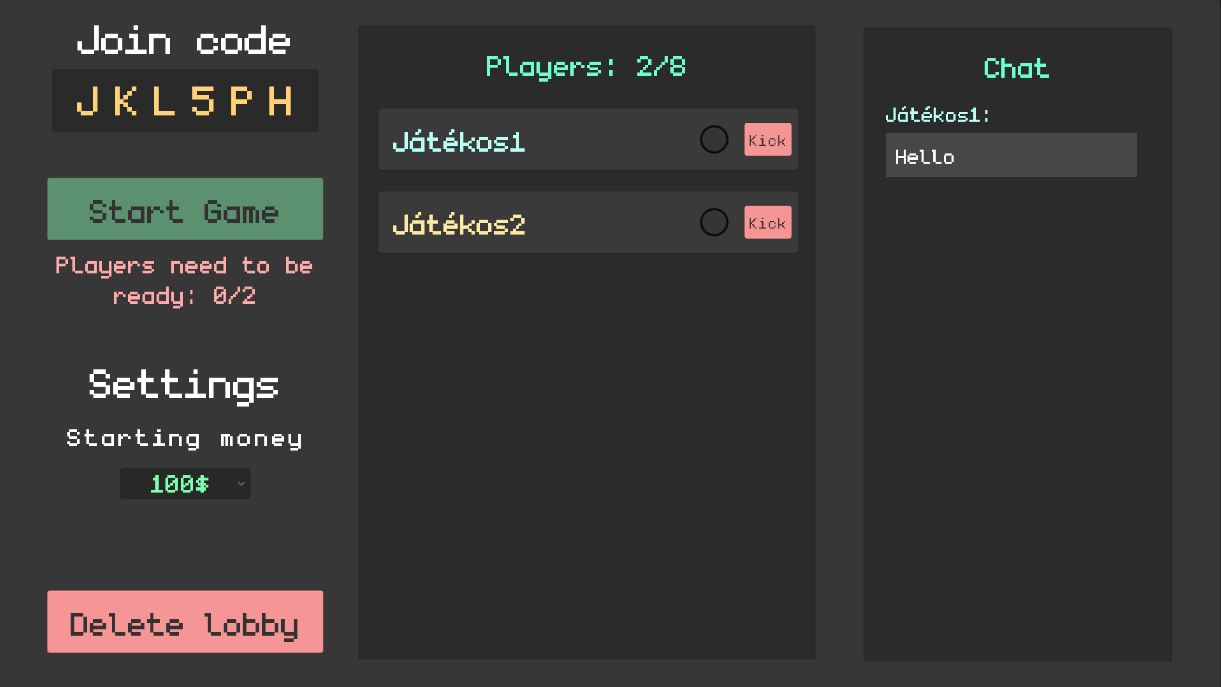
\includegraphics[width=15cm]{Lobby}
	\caption{Lobby jelenet}
	\label{fig-lobby}
\end{figure}

\subsection{Kapcsolat kezelése a Mobil oldalon}

A mobil oldalon a megosztott hozzáférési kód segítségével tudunk csatlakozni a játszmákhoz. A hozzáférési kód megadása mellett egy játékos nevet is kell választatnunk, aminek segítségével később majd a hoszt tud azonosítani minket. Ez a játékos név a sikeres csatlakozás esetén automatikusan egy üzenet formájában el is küldődik a hosztnak. Amennyiben már van ilyen játékos név vagy esetleg már megtelt az adott Lobby, akkor a hoszt küld erről egy tájékoztató üzenetet és ezt lekezelve egy hibaüzenettel vissza térünk a kezdőképernyőre.

Mobil oldalon 2 opciónk van kommunikálni a PC-vel, az egyik az üzenetek küldése a másik pedig a lecsatlakozási kérelem küldése. Az üzenetek küldésére különböző gombok és szöveges dobozok adnak lehetőséget, pl. egy ,,Készen állok'' gomb, ami a Lobby jelenet során jelzi a PC számára, hogy készen állunk a játszma indítására. A játszma során minden egyes lehetséges akciónak az elvégzésekor küldünk egy üzenetet a hosztnak, ami ezt megfelelően kezeli és elküldi a következő játékosnak az ő lehetséges akcióit.

Ha a PC oldalról kapunk egy lecsatlakozási kérelmet, azaz kirúgnak minket egy játszmából, akkor ezt a játék kezeli és egy hibaüzenettel visszatérünk a kezdő képernyőre.

\section{Játékmenet megvalósítása}

A játékmenet fejlesztése során próbáltam figyelni a tiszta és könnyen módosítható kódok és projekt létrehozására. A kód megírása során próbáltam kiszedni absztrakciókba az újból megjelenő funkcionalitásokat, így a jövőben könnyen bővíthető és elkülöníthető kódot tudok írni. A játékfejlesztés során egy bevált módszer az úgymond kezelő szkriptek készítése, ahol egy-egy ilyen kezelő felel egy adott funkcionalitásért, pl. az AudioManager szkript felel a hangokért. Ezeknél a kezelőknél az egyke tervezési mintát használtam, mivel ha szükség van kívülről elérni ezeket a kezelőket, azt így könnyen megtudtam tenni, és biztosította, hogy mindig csak egy kezelő példány legyen létrehozva az adott funkciók kezelésére.

\subsection{Prefab-ek használata}

A fejlesztés során a már \aref{sec-prefab}. fejezetben is említettem hogy a Prefab-ek használata nagyon hasznos tud lenni a többször használatos játék elemek során. A játékban Prefab-et több helyen is használtam, viszont a legfontosabb a játékosokat megjelenítő UI elemek voltak. Ezzel a módszerrel minden játékosnak a megjelenítését egységes módon tudtam kezelni. Ilyen Prefab volt még pl. a hiba üzenetet megjelenítő felugró ablak, a chat üzeneteket megjelenítő chat doboz, a mobilon lévő lehetséges akciókat kezelő gombok és csúszkák és még hasonló UI elemek.

\subsection{Vizuális elemek}

A játék látvány világát leginkább a Unity által szolgáltatott UI elemekből építettem fel. Próbáltam egy pixeles stílust elérni, ezt egy pixeles betűtípus használatával sikerült is egész jól megvalósítanom. A látvány világ kialakításában nagy segítségemre volt a menyasszonyom, Erdész Réka. A játék legfontosabb látványbeli elemei a kártyák és az összes elem aminek a pókerhez van köze Réka által lettek megrajzolva. Ezek az elemek közé tartozik az 52 kártya lap egyedi kinézete, a póker asztal és a póker asztal díszítésére szolgáló póker zsetonok is.

\subsection{Póker játékmenet megvalósítása}

A játékmenet alapját \aref{subsec-pokerszabalyok}. fejezetben leírt szabályok adták. Minden játszma egy frissen kevert 52 lapos paklival kezd, az osztó és a vakok kisorsolásával. A körök logikáját egy szkript kezeli, ahol egy állapotgép alapú megoldás dolgozik háttérben. A körök kezdésekor minden játékos megkapja a tájékoztató üzenetet, arról hogy ki következik, a soron lévő játékos pedig a lehetséges akcióit is megkapja. Miután egy játékos elvégezte az akcióját ezt a PC oldalon a kör kezelő szkript dolgozza fel és a kör állapotától függően a következő játékosnak megint az újra meghatározott lehetséges akciókat ki küldi. Ha egy licit körnek vége van, erről mindenki kap tájékoztatást és a szabályok alapján elindul a következő kör, ez addig megy ameddig csak 1 játékos marad bent a játszmában. Egy játékos kiesik ha a 0\$-t eléri a pénze, ilyenkor egy lecsatlakozási kérelmet és egy üzenetet kap a játékos az elért helyezéséről, amit a mobilon egyből lekezelve látni is fog.

\subsection{Animációk}

Az animációk nagyban segítik a vizuális játékélményt és egyértelműbbé teszi a játékmenet követését. A játékomban ilyen animációk pl. a kártyák osztása, felfordítása és egyéb a játékmenettel kapcsolatos animációk. Az animációk létrehozásához csak kódolást használtam a LeanTween \cite{UnityLeanTween} ingyenesen elérhető csomag segítségével. A LeanTween lehetőséget ad különböző mozgásokat, méretezéseket és forgásokat implementálni a játékelemek részére. Betudjuk állítani a cél tulajdonságon kívül az átmenetet is, ami lehet pl. lineáris, négyzetes és hasonló átmenetek. Az animációk végén (amikor az elemek elérték a cél tulajdonságot), lehetőségünk van callback metódusok segítségével lekezelni ezt az eseményt. Ezeknek a callback metódusoknak köszönhetően könnyen tudtam kezelni az osztás folyamatát, hiszen ha az egyik kártya elérte a célját, akkor el is indíthattam a következő kártyát.

\chapter{Tesztelés}

A tesztelés nagyon fontos része a fejlesztésnek, hiszen ennek a folyamatnak a során tárjuk fel a lehetséges hibákat a programunkban. A tesztek nagy szerepet játszanak az egyszerűen bővíthető és fejleszthető kódbázisokban, hiszen így minden módosítás és bővítés után letudjuk ellenőrizni, hogy van-e hiba a kódban. A legelterjedtebb tesztelési forma az \emph{egység tesztek} írása, ahol 1-1 metódusnak vagy függvénynek több különböző bemenet alapján vizsgáljuk a várt kimenetét. Az egység tesztek során le kezeljük a helyes bemenetre való működést és az akár hibát kiváltó bemenetre való működést is. 

Az egyik legfontosabb tesztelési módszer játékfejlesztés szempontjából a játék teszt (playtest), ahol a játékot minél körültekintőbben játszva tárjuk fel az esetleges hibákat és teszt jegyzőkönyveket vezetünk ezeknek a teszteknek a menetéről. Fontos lehet hogy ezeket a játék teszteket ne csak önmagunk csináljuk hiszen mi ismerjük a játékot és akár azok a részek amik nem egyértelműek első felhasználói szempontból nekünk nem biztos hogy feltűnnek. Külsős tesztelők sok olyan dolgot fedezhetnek fel, ami nekünk eszünkbe se jutott volna de mégis sokat javít a játékélmény növelésében.

A tesztelés folyamatát az is segítheti egy ekkora projektnél, hogy megpróbálunk minél tisztább és rendezettebb kódot írni, így az egység teszteket is egyszerűbb dolgunk lesz megírni. A tiszta kód írásának egyik módja lehet az OOP (Objektum orientált programozás) alapelveinek betartása lehet.

\section{Közös DLL tesztelése}

A közös DLL tesztelése során a már fentebb említett egység teszteket alkalmaztam. A kódban lévő összes metódusra és függvényre írtam egység teszteteket, minden lehetséges eset tesztelésére. Ezeknek a teszteknek a segítségével könnyen tudtam bővíteni és ellenőrizni a kódbázist. Mint, ahogy korábban \aref{sec-architecture}. fejezetben említettem a közös DLL projektnek az egyik legfontosabb része a kézkiértékelést kezelő algoritmus. A kézkiértékeléshez írt egység teszteknél különösen figyeltem arra, hogy minden lehetséges pókerkéz kombinációt használjak bemenetként és az esetleges döntetlen eseteket is figyelembe vettem.

\section{Játékok tesztelése}

A játékok tesztelésében legnagyobb szerepet a playtest játszott, amit már egészen a korai fejlesztési fázisban is elkezdtem. A playtest-ek kétféleképpen néztek ki:

\begin{itemize}
	\item Barátokkal: a ki buildelt Unity játékokat élesben teszteltük közösen. Ezeknél a teszteknél a hibák feltárása mellet sok visszajelzést kaptam, amik segítettek a játékélmény fejlesztését. Ezek a tesztek egy kis motivációs lendületet is tudtak adni, hiszen jó volt látni ahogy a barátaim élvezik a játékot, akár még hibás állapotában is.
	\item Egyedül: a Unity editor által adott lehetőségeket kihasználva teszteltem a játékot. Ez azt jelentette, hogy a PC játék 1 példányban futott a gépemen, a mobil játék pedig a Unity által szolgáltatott \emph{Multiplayer play mode}-nak köszönhetően egyszerre 2-4 példányban futott a gépemen. Ezeknek a teszteknek a során a hibák keresésére fókuszáltam \cite{UnityMultiplayerPlayMode}.
\end{itemize}

A playtest-ek során mindig odafigyeltem, hogy minden lehetőséget kipróbáljak a játékban. Ezek a playtest-ek nem csak hibakeresésre de játékélménybeli javításába is sokat segítettek, hiszen a barátaim sok dolgot észrevettek és jeleztek felém, amik a játékélményt segíthetik. Későbbiekben készítettem egy naplózó rendszert is a játékokhoz, ami megkönnyítette a hibák feltárását.

Mindkét játékhoz készítettem a már korábbiakban említett egység teszteket is, amikhez az NUnit könyvtárat használtam. Játékfejlesztés során körülményes lehet az egység tesztek használata, hiszen nagyon sokszor egy adott kódrészlet akár több másik komponenstől is függhet, ennek megoldására úgynevezett mock komponenseket hozunk létre. A Mock komponensek segítségével a hiányzó függőségeket betudjuk tölteni a tesztelendő osztályban \cite{NUnit}.

\subsubsection{Teszt jegyzőkönyv}

A playtest-ek során teszt jegyzőkönyvet vezettem. A jegyzőkönyvek segítettek a hibák dokumentálásában, így később is egységes formában át tudtam nézni az észlelt hibákat. Egy ilyen jegyzőkönyv látható a főmenü jelentről \aref{tab-tesztjegyzokonyv}. táblázatban. A jelenetekre mindig külön jegyző könyveket vezettem, a könnyebb átláthatóság érdekében.

\begin{table}[ht!]
	\centering
	\footnotesize
	\begin{tabular}{|c|c|c|c|}
		\hline
		\textbf{Időpont} & \textbf{Teszt} & \textbf{Eredmény} & \textbf{Megjegyzés} \\
		\hline
		22:01 & Indítás gomb & Sikeres & Betölti a Lobby jelenetet \\
        \hline
		22:03 & Kilépés gomb & Sikeres & Kilép a játékból \\
		\hline
		22:10 & Beállítások gomb & Sikeres & Betölti a beállítások felületet \\
		\hline
		22:12 & Beállítások bezárása gomb & Sikeres & Bezárja a beállítások felületet \\
		\hline
		22:15 & Felbontás módosítása & Sikeres & A felbontásokat helyesen felsorolj \\
		\hline
		22:18 & Minőség módosítása & Sikeres & A minőségeket helyesen felsorolja \\
		\hline
		22:20 & Képernyőmód módosítása & Sikeres & Ablakos és teljes képernyő közötti váltás \\
		\hline
		22:23 & SFX hangerő módosítása & Sikeres & Csúszkával lehet módosítani az értékét. \\
		\hline
		22:25 & Zene hangerő módosítása & Sikeres & Csúszkával lehet módosítani az értékét \\
		\hline
		22:30 & Beállítások elfogadása & Sikeres & Módosítja a változtatott beállításokat \\
		\hline
	\end{tabular}
	\caption{Példa tesztjegyzőkönyv a főmenüről (2024.12.28)}
	\label{tab-tesztjegyzokonyv}
\end{table}

\pagebreak

A tesztelés folyamata lehet körülményes és néhány helyen érződhet úgy hogy csak idő pazarlás, de mindenképpen megéri időt tölteni vele. A játékfejlesztésben pedig a hibakeresésen kívül másban is fontos szerepet játszik, hiszen akár a játékélmény fejlesztésében is segíthet. Vannak olyan játékok is, ahol a játékmenet kiegyensúlyozásának érdekében is rákényszerülünk a tesztelésre és elhagyhatatlan eleme a fejlesztési folyamatnak. Az én játékom esetében hiba keresésben és játékélménybeli javításban is sokat segítettek a fentebb említett tesztelési módszerek.

\chapter*{Összegzés}
\addcontentsline{toc}{chapter}{Összegzés}

A szakdolgozatom során sikerült teljesítenem az előre kitűzött elvárásokat. Ezek az elvárások és követelmények \aref{ch-rendszerterv}. fejezetben részletesen megjelennek. Sikeresen megvalósítottam a kapcsolatot a két platform között és összességében sikerült könnyen kezelhető és bővíthető kódot írnom a játék fejlesztése során. A későbbiekben a tisztán tartott kódbázisnak köszönhetően a bővítés nagyobb átalakítások nélkül is megvalósulhat.

\section{Bővítési terv}

A játékmenet bővítésére 2 jelentősebb tervet említek meg ebben a szekcióban. Az egyik ilyen terv a mesterséges intelligencia implementálása, játékos létszám növelésének érdekében. Ez azt jelentené, hogy a felcsatlakozott játékosokon kívül ,,bot'' játékosokat lehetne hozzáadni a játszmákhoz, amit a háttérben mesterséges intelligencia irányítana. A másik ilyen terv pedig különböző ismert kártyajátékok, akár póker variációk hozzáadása a játékhoz. Ezeket a terveket mindenképp megszeretném valósítani a későbbiekben, sok-sok más egyéb fejlesztéssel együtt a játékélmény növelésének érdekében.

\section{Konklúzió}

A játék fejlesztése során sok újat tanultam a Unity keretrendszerben történő fejlesztésről. Az előző projektjeim alapján már alapból elég jól ismertem a keretrendszert, de egy ilyen nagyobb szabású projekt során sok olyan elem és technológia került elő amivel eddig nem találkoztam. Sikerült teljesítenem a többjátékos játék fejlesztése célomat is, és a továbbiakban sokkal magabiztosabban tudok ilyen fejlesztésbe kezdeni.

\begin{center}
	Forráskód elérhetősége:
	
	{\color{teal}\url{https://github.com/szbmrk/H8P190_Thesis}}
	
	Játék elérhetősége:
	
	{\color{teal}\url{https://pokerparty.szobo.dev}}
	
	Bemutató videó elérhetősége:
	
	{\color{teal}\url{https://youtu.be/Zxf-6lE1qjM}}
\end{center}

\chapter*{Ábrák jegyzéke}
\addcontentsline{toc}{chapter}{Ábrák jegyzéke}

\ref{fig-clientserver}. ábra -- saját készítésű ábra, \cite{ResearchGateClientServer} alapján
\newline
\ref{fig-p2p}. ábra -- saját készítésű ábra, \cite{TechTermsP2P} alapján
\newline
\ref{fig-unityeditor}. ábra -- saját készítésű ábra
\newline
\ref{fig-unityrelayservers}. ábra -- saját készítésű ábra, \cite{UnityRelayServers} alapján
\newline
\ref{fig-pokerhands}. ábra -- forrás: \url{https://cardmates.co.uk/all_poker_hands} [Letöltve: 2025-03-02]  
\newline
\ref{fig-lobby}. ábra -- saját készítésű ábra

\begin{thebibliography}{2}
	\addcontentsline{toc}{chapter}{\bibname}
	
	\bibitem{UnrealEngine}
	\textsc{Epic Games}: \emph{Unreal Engine}, elérhető: \url{https://www.unrealengine.com} [Letöltve: 2025-02-28]
	
	\bibitem{Godot}
	\textsc{Juan Linietsky, Ariel Manzur, Godot közösség}: \emph{Godot}: \url{https://godotengine.org} [Letöltve: 2025-02-28]
	
	\bibitem{GitHubGodot}
	\textsc{GitHub}: \emph{Godot}: \url{https://github.com/godotengine/godot} [Letöltve: 2025-02-28]
	
	\bibitem{Unity}
	\textsc{Unity Technologies}: \emph{Unity}, elérhető: \url{https://unity.com} [Letöltve: 2025-02-28]
	
	\bibitem{MediumMultiplayer}
	\textsc{Jamal Aladdin}: \emph{The Evolution of Multiplayer Gaming: A Journey Through Time}, Jamal Aladdin blogja, elérhető: \href{https://medium.com/@Jamal_Aladdin/the-evolution-of-multiplayer-gaming-a-journey-through-time-e34ef59294c2}{Jamal Aladdin blogja} [Letöltve: 2025-02-28]
	
	\bibitem{MediumClientServer}
	\textsc{Lem Apperson}: \emph{Beginning Game Development: Client-Server Architecture}, Lem Apperson blogja, elérhető:
	\url{https://medium.com/@lemapp09/beginning-game-development-client-server-architecture-1b7676d80dea} [Letöltve: 2025-02-28]
	
	\bibitem{ResearchGateClientServer}
	\textsc{T.C Nicholas Graham}: \emph{Figure1}, elérhető:
	\href{https://www.researchgate.net/figure/Typical-client-server-architecture-server-maintains-canonical-game-state-local-clients_fig1_262275278}{Figure 1 - Client-Server} [Letöltve: 2025-04-02]
	
	\bibitem{MediumP2P}
	\textsc{Tashi Protocol}: \emph{Peer-to-Peer Gaming}, Tashi Protocol blogja, elérhető:
	\url{https://medium.com/tashi-gg/peer-to-peer-gaming-9991600c6707} [Letöltve: 2025-03-02]
	
	\bibitem{TechTermsP2P}
	\textsc{TechTerms}: \emph{P2P}, elérhető:
	\url{https://techterms.com/definition/p2p} [Letöltve: 2025-04-02]
	
	\bibitem{UnityPlatforms}
	\textsc{Unity Technologies}: \emph{Platform development}, elérhető:
	\url{https://docs.unity3d.com/Manual/PlatformSpecific.html} [Letöltve: 2025-03-03]
	
	\bibitem{Unity6Features}
	\textsc{Martin Best}: \emph{Unity 6 is here: See what's new}, elérhető:
	\url{https://unity.com/blog/unity-6-features-announcement} [Letöltve: 2025-03-03]
	
	\bibitem{UnityScene}
	\textsc{Unity Technologies}: \emph{Scenes}, elérhető:
	\url{https://docs.unity3d.com/560/Documentation/Manual/CreatingScenes.html} [Letöltve: 2025-03-03]
	
	\bibitem{UnityGameObjects}
	\textsc{Unity Technologies}: \emph{GameObjects}, elérhető:
	\url{https://docs.unity3d.com/560/Documentation/Manual/GameObjects.html} [Letöltve: 2025-03-03]
	
	\bibitem{UnityComponents}
	\textsc{Unity Technologies}: \emph{Using Components}, elérhető:
	\url{https://docs.unity3d.com/560/Documentation/Manual/UsingComponents.html} [Letöltve: 2025-03-03]
	
	\bibitem{UnityTransform}
	\textsc{Unity Technologies}: \emph{Transform}, elérhető:
	\url{https://docs.unity3d.com/560/Documentation/Manual/class-Transform.html} [Letöltve: 2025-03-03]
	
	\bibitem{UnityRigidbody}
	\textsc{Unity Technologies}: \emph{RigidBody}, elérhető:
	\url{https://docs.unity3d.com/Manual/class-Rigidbody.html} [Letöltve: 2025-03-03]
	
	\bibitem{UnityCamera}
	\textsc{Unity Technologies}: \emph{Camera}, elérhető:
	\url{https://docs.unity3d.com/6000.0/Documentation/ScriptReference/Camera.html} [Letöltve: 2025-03-03]
	
	\bibitem{UnityCollider}
	\textsc{Unity Technologies}: \emph{Collider}, elérhető:
	\url{https://docs.unity3d.com/6000.0/Documentation/ScriptReference/Collider.html} [Letöltve: 2025-03-03]
	
	\bibitem{UnitySpriteRenderer}
	\textsc{Unity Technologies}: \emph{Sprite Renderer}, elérhető:
	\url{https://docs.unity3d.com/540/Documentation/Manual/class-SpriteRenderer.html} [Letöltve: 2025-03-03]
	
	\bibitem{UnityLight}
	\textsc{Unity Technologies}: \emph{Light}, elérhető:
	\url{https://docs.unity3d.com/6000.0/Documentation/ScriptReference/Light.html} [Letöltve: 2025-03-03]
	
	\bibitem{UnityAudioSource}
	\textsc{Unity Technologies}: \emph{Audio Source}, elérhető:
	\url{https://docs.unity3d.com/Manual/class-AudioSource.html} [Letöltve: 2025-03-03]
	
	\bibitem{UnityScripting}
	\textsc{Unity Technologies}: \emph{Scripting}, elérhető:
	\url{https://docs.unity3d.com/Manual/scripting.html} [Letöltve: 2025-03-03]
	
	\bibitem{UnityPrefab}
	\textsc{Unity Technologies}: \emph{Prefabs}, elérhető:
	\url{https://docs.unity3d.com/Manual/Prefabs.html} [Letöltve: 2025-03-03]
	
	\bibitem{UnityProjectWindow}
	\textsc{Unity Technologies}: \emph{The Project Window}, elérhető:
	\url{https://docs.unity3d.com/6000.0/Documentation/Manual/ProjectView.html} [Letöltve: 2025-03-03]
	
	\bibitem{UnitySceneView}
	\textsc{Unity Technologies}: \emph{The Scene View}, elérhető:
	\url{https://docs.unity3d.com/6000.0/Documentation/Manual/UsingTheSceneView.html} [Letöltve: 2025-03-03]
	
	\bibitem{UnityHierarchyWindow}
	\textsc{Unity Technologies}: \emph{The Hierarchy Window}, elérhető:
	\url{https://docs.unity3d.com/6000.0/Documentation/Manual/Hierarchy.html} [Letöltve: 2025-03-03]
	
	\bibitem{UnityInspectorWindow}
	\textsc{Unity Technologies}: \emph{The Inspector Window}, elérhető:
	\url{https://docs.unity3d.com/6000.0/Documentation/Manual/UsingTheInspector.html} [Letöltve: 2025-03-03]
	
	\bibitem{UnityGameView}
	\textsc{Unity Technologies}: \emph{The Game View}, elérhető:
	\url{https://docs.unity3d.com/6000.0/Documentation/Manual/GameView.html} [Letöltve: 2025-03-03]
	
	\bibitem{UnityRelayService}
	\textsc{Unity Technologies}: \emph{Relay: Free P2P Networking \& Connection Solution}, elérhető:
	\url{https://unity.com/products/relay} [Letöltve: 2025-03-04]
	
	\bibitem{UnityRelayDocs}
	\textsc{Unity Technologies}: \emph{Unity Relay}, elérhető:
	\url{https://docs.unity.com/ugs/manual/relay/manual/introduction} [Letöltve: 2025-03-04]
	
	\bibitem{UnityRelayServers}
	\textsc{Unity Technologies}: \emph{Relay Servers}, elérhető:
	\url{https://docs.unity.com/ugs/en-us/manual/relay/manual/relay-servers} [Letöltve: 2025-03-04]
	
	\bibitem{UnityAllocationsService}
	\textsc{Unity Technologies}: \emph{Allocations Service}, elérhető:
	\url{https://docs.unity.com/ugs/en-us/manual/relay/manual/allocations-service} [Letöltve: 2025-03-04]
	
	\bibitem{Rider}
	\textsc{JetBrains}: \emph{Rider}, elérhető:
	\url{https://www.jetbrains.com/rider/} [Letöltve: 2025-03-07]
	
	\bibitem{Git}
	\textsc{Linus Torvalds, Junio Hamano}: \emph{Git}, elérhető:
	\url{https://git-scm.com/} [Letöltve: 2025-03-07]
	
	\bibitem{GitHub}
	\textsc{GitHub, Inc.}: \emph{GitHub}, elérhető:
	\url{https://github.com/} [Letöltve: 2025-03-07]
	
	\bibitem{Trello}
	\textsc{Atlassian}: \emph{Trello}, elérhető:
	\url{https://trello.com/} [Letöltve: 2025-03-07]
	
	\bibitem{TexasholdemSzabalyok}
	\textsc{PokerStrategy}: \emph{A Texas hold'em játékszabályai
	}, elérhető: \url{	https://hu.pokerstrategy.com/strategy/various-poker/texas-holdem-jatekszabalyok} [Letöltve: 2024-11-13]
	
	\bibitem{HandEvaluation}
    \textsc{Jonathan Hsiao}: \emph{Evaluating Poker Hands with Bit Math}, Jonathan Hsiao blogja, elérhető: \url{https://jonathanhsiao.com/blog/evaluating-poker-hands-with-bit-math} [Letöltve: 2025-02-25]
	
	\bibitem{Szurdi}
	\textsc{Szurdi András}: \emph{Pókerkönyv. Kezdőknek és haladóknak}, Ciceró, Budapest, 1995.
	
	\bibitem{Varga}
	\textsc{Varga Ervin}: \emph{Póker alapkönyv}, Vagabund, Kecskemét, 2008.
	
	\bibitem{UnityLeanTween}
	\textsc{DentedPixel}: \emph{LeanTween}, dokumentáció elérhető:
	\url{https://dentedpixel.com/LeanTweenDocumentation/classes/LeanTween.html} [Letöltve: 2025-03-11]
	
	\bibitem{UnityMultiplayerPlayMode}
	\textsc{Unity Technologies}: \emph{Multiplayer Play Mode}, elérhető:
	\url{https://docs.unity3d.com/6000.0/Documentation/Manual/com.unity.multiplayer.playmode.html} [Letöltve: 2025-03-03]
	
	\bibitem{NUnit}
	\textsc{NUnit}: a unit-testing framework for all .Net languages, elérhető: \url{https://docs.nunit.org/} [Letöltve: 2025-03-02]
	
\end{thebibliography}

% Aláírt, szkennelt nyilatkozat beillesztése a szakdolgozat végére
%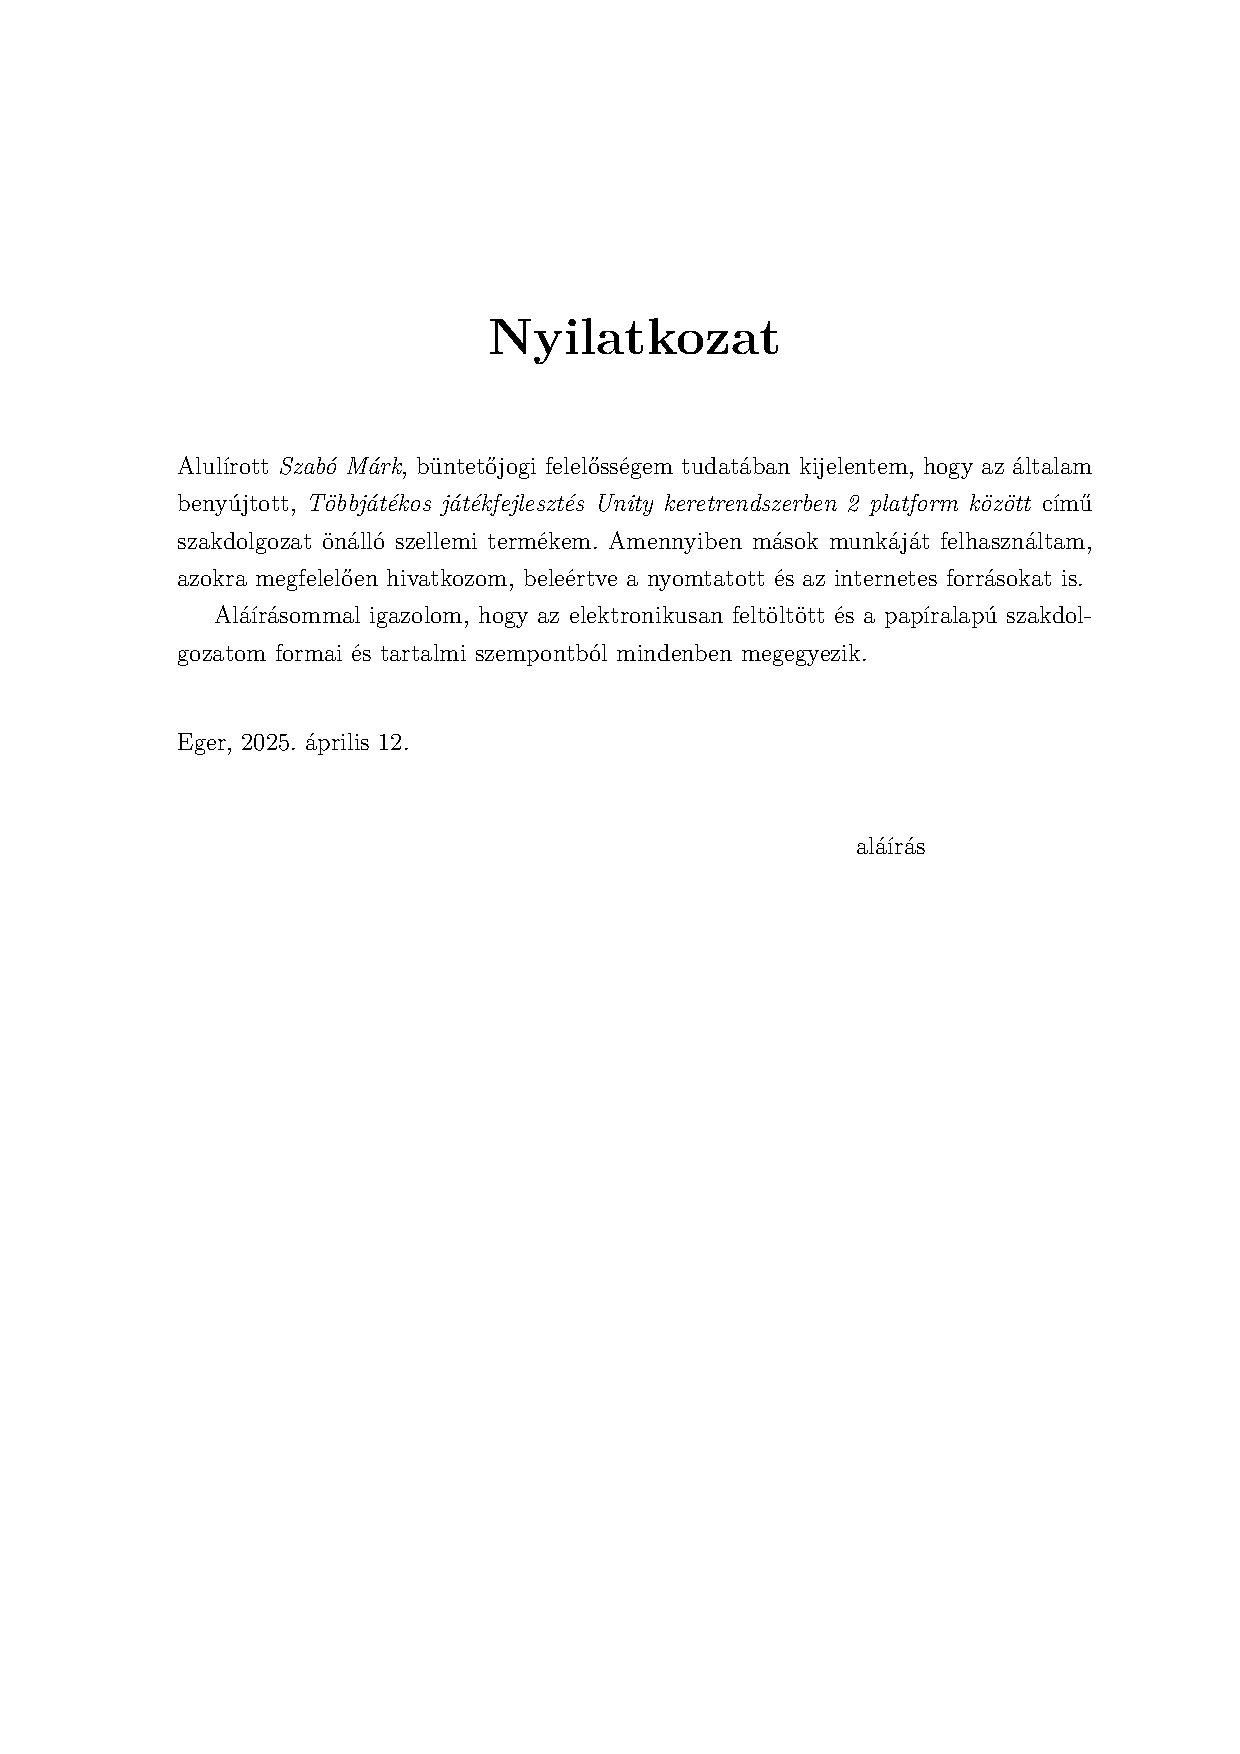
\includepdf{nyilatkozat/nyilatkozat.pdf}

\end{document}